% document type: science report
\documentclass[abstracton, a4paper, 12pt]{scrreprt}

% Encoding (utf8)
\usepackage[utf8]{inputenc}
\usepackage[T1]{fontenc}

% Silbentrennung (Neu-Deutsch)
\usepackage[ngerman]{babel}

% Literaturverzeichnis (Deutsch)
\usepackage{bibgerm}

% Farben
\usepackage{color}
\usepackage[table]{xcolor}
\definecolor{darkgreen}{rgb}{0,0.6,0}
\definecolor{darkgrey}{rgb}{0.5,0.5,0.5}
\definecolor{grey}{rgb}{0.8,0.8,0.8}
\definecolor{lightgrey}{rgb}{0.95,0.95,0.95}
\definecolor{mauve}{rgb}{0.58,0,0.82}

% Grafiken
\usepackage[pdftex]{graphicx}
\usepackage{epsfig}
% Umfliessen von Text um Tabellen und Bilder
\usepackage{wrapfig}

% Grafiken korrekt positionieren
\usepackage{float}
\restylefloat{figure}
\usepackage[section]{placeins}
\usepackage{subfigure}

% hyperlinks
\usepackage{hyperref}
\hypersetup{
   colorlinks,%
   citecolor=blue,%
   filecolor=blue,%
   linkcolor=blue,%
   urlcolor=blue
}
\urlstyle{same}

% Absatz
\setlength{\parindent}{0pt} % Absatzeinzug
\setlength{\parskip}{10pt} % Absatzabstand

% Glossar
\usepackage[toc]{glossaries}
\makeglossaries

% TODO Kommentare
\usepackage{todonotes}

% Definition vom Header und Footer im Seitenlayout
\usepackage{fancyhdr} 
\pagestyle{fancy} 
\fancyhf{}

% Linien nach dem Header und vor dem Footer
%\renewcommand{\footrulewidth}{0.4pt}
%\renewcommand{\headrulewidth}{0.4pt}

\fancyhead[L]{\footnotesize{\leftmark}}
\fancyfoot[C]{\footnotesize{\thepage}}
\fancyhead[R]{}

% Header auch bei Kapitelanfangsseite
\def\chapterpagestyle{fancy}

% Tabelle
% Padding links und rechts von Zelle
\setlength{\tabcolsep}{5px}
% Padding oben und unten (mittels arraystretch)
\renewcommand{\arraystretch}{1.3}

% Für schöne URLs
\usepackage{url}

% Syntaxhighlighter (benoetigt color und xcolor package)
\usepackage{listings}
 
\lstset{ %
  language=HTML,                % the language of the code
  basicstyle=\footnotesize,           % the size of the fonts that are used for the code
  numbers=left,                   % where to put the line-numbers
  numberstyle=\tiny\color{darkgrey},  % the style that is used for the line-numbers
  stepnumber=1,                   % the step between two line-numbers. If it's 1, each line will be numbered
  numbersep=5pt,                  % how far the line-numbers are from the code
  backgroundcolor=\color{white},  % choose the background color. You must add \usepackage{color}
  showspaces=false,               % show spaces adding particular underscores
  showstringspaces=false,         % underline spaces within strings
  showtabs=false,                 % show tabs within strings adding particular underscores
  frame=single,                   % adds a frame around the code
  rulecolor=\color{darkgrey},        % if not set, the frame-color may be changed on line-breaks within not-black text (e.g. commens (green here))
  tabsize=2,                      % sets default tabsize to 2 spaces
  captionpos=b,                   % sets the caption-position to bottom
  breaklines=true,                % sets automatic line breaking
  breakatwhitespace=false,        % sets if automatic breaks should only happen at whitespace
  title=\lstname,                   % show the filename of files included with \lstinputlisting;
                                  % also try caption instead of title
  keywordstyle=\color{blue},          % keyword style
  commentstyle=\color{darkgreen},       % comment style
  stringstyle=\color{mauve},         % string literal style
  escapeinside={\%*}{*)},            % if you want to add a comment within your code
  morekeywords={*,...}               % if you want to add more keywords to the set
}

% Javascript Syntaxhighliting
\lstdefinelanguage{JavaScript} {
	morekeywords={
		break,const,continue,delete,do,while,export,for,in,function,
		if,else,import,in,instanceOf,label,let,new,return,switch,this,
		throw,try,catch,typeof,var,void,with,yield
	},
	sensitive=false,
	morecomment=[l]{//},
	morecomment=[s]{/*}{*/},
	morestring=[b]",
	morestring=[d]'
}
\lstset{
	frame=tb,
	framesep=5pt,
	basicstyle=\footnotesize\ttfamily,
	showstringspaces=false,
	keywordstyle=\ttfamily\bfseries\color{blue},
	identifierstyle=\ttfamily,
	stringstyle=\ttfamily\color{mauve},
	commentstyle=\color{darkgreen},
	rulecolor=\color{darkgrey},
	xleftmargin=5pt,
	xrightmargin=5pt,
	aboveskip=\bigskipamount,
	belowskip=\bigskipamount
}

%% define toc formatting
%\usepackage[titles]{tocloft}
%\setlength{\cftsubsecindent}{3em}
%\setlength{\cftsubsecnumwidth}{3.3em}
%\setlength{\cftsubsubsecindent}{4.5em}
%\setlength{\cftsubsubsecnumwidth}{4em}

%% figure numbering
%\newcounter{myfigure}
%\renewcommand{\thefigure}{\arabic{myfigure}}
%\newcounter{mytable}
%\renewcommand{\thetable}{\arabic{mytable}}
%\usepackage{makeidx} \makeindex
%\makeglossary

%% Definition vom Seitenlayout
%\setlength{\topmargin}{-1.2cm}
%\setlength{\oddsidemargin}{0.5cm} 
%\setlength{\evensidemargin}{0.5cm}

%\setlength{\textheight}{24.5cm} 
%\setlength{\textwidth}{15cm}

%\setlength{\footskip}{1.2cm} 
%\setlength{\footnotesep}{0.4cm}

%% Neues Kapitel Makro, damit die Variablen korrekt abgefuellt werden
%\newcommand{\newchap}[1]{
%	\chapter{#1}
%	\markboth {Kapitel \thechapter.  {#1}}{Kapitel \thechapter.  {#1}}
%}
%
%% command to import a figure
%\newcommand{\fig}[5]{
%  \begin{figure}[h]
%    \begin{center}
%      \includegraphics[width=#4cm]{#1}
%    \end{center}
%    \stepcounter{myfigure}
%    \caption[#5]{#3}
%    \label{#2}
%  \end{figure}
%}
%
%\newcommand{\figtable}[4]{
%  \begin{figure}[h]
%    \begin{center}
%      {  
%			  \footnotesize
%  			\sffamily
%			  #3
%      }
%    \end{center}
%    \stepcounter{myfigure}
%    \caption[#4]{#2}
%    \label{#1}
%  \end{figure}
%}
%
%\newcommand{\tab}[4]{
%  \begin{table}[h]
%    \begin{center}
%      {  
%			  \footnotesize
%  			\sffamily
%  			\renewcommand{\arraystretch}{1.4}
%			  #3  			
%      }
%    \end{center}
%    \stepcounter{mytable}
%    \caption[#4]{#2}
%    \label{#1}
%  \end{table}
%}
%
%% command to refere to a figure
%\newcommand{\reffig}[1]{Abbildung \ref{#1}}
%
%% Definition des Nummerierungslevel
%\setcounter{secnumdepth}{4} 
%\setcounter{tocdepth}{4} 
%\setcounter{lofdepth}{1} 
%
%% Definition von Paragraphen
%\parskip=0.3cm
%\parindent=0cm
%
%% Definition vom Zeilenabstand
%\usepackage{setspace} % Zeilenabstand
%\onehalfspacing
%
%% Befehle fuer Anfuehrungszeichen
%\usepackage{xspace} % Leerschlag nach Anfuehrungszeichen
%\newcommand{\qr}{\grqq\xspace}
%\newcommand{\qrs}{\grqq\ }
%\newcommand{\ql}{\glqq}
%
%% Formatierungsbefehle zum Zitieren
%\newcommand{\page}[1]{S.~#1}
%\newcommand{\pagef}[1]{S.~#1f.}
%\newcommand{\pageff}[1]{S.~#1ff.}
%\newcommand{\pages}[2]{S.~#1--#2}

\begin{document}

% -----------------------------------------
% HEAD
% -----------------------------------------
% Titelseite
\title{Cloudbasiertes Geodatenmanagement mit Google Fusion Tables}
\author{Jürg Hunziker\\jhunzike@hsr.ch
		\and
		Stefan Oderbolz\\soderbol@hsr.ch}
\date{29. Mai 2012}

\begin{titlepage}

% Logos

\includegraphics[width=200px]{./images/logo-hsr}
\hfill
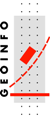
\includegraphics[width=40px]{./images/logo-geoinfo}
\vspace{2.2cm}

\begin{center}
{ \Large
	% Titel
	\textbf{Cloudbasiertes Geodatenmanagement mit Google Fusion Tables: Entwicklung eines Cloud-GIS Prototypen}
	\vspace{1cm}

	% Arbeitstyp / Schule
	\textbf{Studienarbeit}
	\vspace{1cm}

	Abteilung Informatik \\[0.2cm]
	Hochschule für Technik Rapperswil
	\vspace{1cm}

	% Semester
	Frühjahrssemester 2012
}
\end{center}
\vspace{2.3cm}

\begin{tabular}{p{0.19\twocelltabwidth}p{0.81\twocelltabwidth}}
Autoren: & \textbf{Stefan Oderbolz} (\url{soderbol@hsr.ch}) \newline
 \textbf{Jürg Hunziker} (\url{jhunzike@hsr.ch}) \\ 
Betreuer: & \textbf{Prof. Stefan Keller} (\url{sfkeller@hsr.ch}) \\ 
Projektpartner: & \textbf{Marco Lehmann}, GEOINFO AG Herisau, \url{http://www.geoinfo.ch} \\ 
Experte: & \textbf{Prof. Stefan Keller} (\url{sfkeller@hsr.ch}) \\ 
Datum: & \textbf{29. Mai 2012} \\ 
\end{tabular}

\end{titlepage}

% Seitennummerierung mit roemischen Zeichen
\pagenumbering{roman}

% Glossar (muss vor Body inkludiert werden, damit Referenzen funktionieren)
% Glossar
\newglossaryentry{Geocodierung} {
name = Geocodierung,
description = {Bei der Geocodierung wird eine Zeichenkette (Adresse, Namen) einer geografischen Position zugewiesen.}
}


% TODO Liste
% Titel auch in Kopfzeile anzeigen
%\markboth{Todo list}{Todo list}
%\listoftodos

% Impressum & Aenderungsverlauf
\chapter*{Impressum und Revision}
% Titel auch in Kopfzeile anzeigen
\markboth{Impressum und Revision}{Impressum und Revision}

% Impressum
\section*{Impressum}
\begin{longtable}{|l|p{11cm}|}
\hline 
\textbf{Autoren:} & Stefan Oderbolz (\url{soderbol@hsr.ch}) \newline
Jürg Hunziker (\url{jhunzike@hsr.ch}) \\ 
\hline 
\textbf{Dokument erstellt:} & 27.02.2012 \\ 
\hline 
\textbf{Letzte Aktualisierung:} & 29.05.2012 \\ 
\hline 
\end{longtable}

% Aenderungsverlauf
\section*{Änderungsverlauf}

\begin{longtable}{|p{2cm}|p{10cm}|p{3cm}|}
\hline 
\textbf{Datum} & \textbf{Änderungen} & \textbf{Bearbeiter} \\ 
\hline 
27.02.2012 & Dokumententwurf erstellt & Stefan Oderbolz \\ 
\hline 
01.03.2012 & Struktur erstellt & Jürg Hunziker \\ 
\hline 
09.03.2012 & Weitergearbeitet an Einleitung & Jürg Hunziker \\ 
\hline 
05.04.2012 & Mit Dokumentation des Use Cases 1: WorldData begonnen & Jürg Hunziker \\ 
\hline 
06.04.2012 & Benutzerdokumentation erstellt für den Use Cases 1: WorldData & Jürg Hunziker \\ 
\hline 
09.04.2012 & Bildbeschriftungen zu bestehenden Grafiken hinzugefügt & Jürg Hunziker \\ 
% revisions from git
\hline 
\end{longtable} 

% Erklaerung
\chapter*{Erklärung}
% Titel auch in Kopfzeile anzeigen
\markboth{Erklärung}{Erklärung}

Ich erkläre hiermit,
\begin{itemize}
\item dass ich die vorliegende Arbeit selber und ohne fremde Hilfe durchgeführt habe, ausser derjenigen, welche explizit in der Aufgabenstellung erwähnt ist oder mit dem Betreuer schriftlich vereinbart wurde,
\item dass ich sämtliche verwendeten Quellen erwähnt und gemäss gängigen wissenschaftlichen Zitierregeln korrekt angegeben habe.
\end{itemize}

\vspace{3cm}

\begin{tabular}{p{0.5\twocelltabwidth}p{0.5\twocelltabwidth}}
Ort, Datum: & Ort, Datum: \\ 
\end{tabular} 

\vspace{1cm}

\begin{tabular}{p{0.5\twocelltabwidth}p{0.5\twocelltabwidth}}
Name, Unterschrift: & Name, Unterschrift: \\ 
\end{tabular} 

% Abstract
% Titel des Abstracts aendern
\renewcommand{\abstractname}{{\Huge\bfseries Abstract}}

\begin{abstract}
% Seitennummerierung auf Abstract-Seite einschalten
\thispagestyle{plain}

Ziel dieser Arbeit war es das Potentials der Cloud-Datenbank \emph{Goolge Fusion Tables} aufzuzeigen. Dazu wurden zuerst einige Beispiele erstellt, welche die verschiedenen Features der Fusion Table verwenden. Zusätzlich wurden Anwendungsfälle im GIS-Bereich gesucht, welche sich ebenfalls mit Google Fusion Tables umsetzen lassen würden. Diese wurden dann als Prototypen implementiert, um den Aufwand aufzuzeigen, welchen es benötigt, um mit Google Fusion Tables eine GIS-Software zu entwickeln.

Es wurden schlussendlich zwei Anwendungsfälle umgesetzt. Zum einen wurde eine Webapplikation implementiert, die es erlaubt historische Daten von verschiedenen Ländern miteinander zu vergleichen. Das Ziel dabei, war das Anzeigen von grossen Datenmengen auf der Karte.

Als zweiten Anwendungsfall wurde eine mobile WebApp entwickelt, welche es dem Benutzer erlaubt Defekte in seiner Umgebung an die zuständige Behörde zu melden. Google Fusion Table wurde dabei als Datenbank zur Speicherung der gemeldeten Defekte verwendet.
\end{abstract}

% Management Summary / Web-Publikation
\chapter*{Management Summary und Web-Publikation}
% Titel auch in Kopfzeile anzeigen
\markboth{Management Summary und Web-Publikation}{Management Summary und Web-Publikation}

\todo[inline]{Management Summary erstellen}
Das Management Summary soll 2-5 Seiten umfassen sowie eine bis zwei Figuren enthalten. Es richtet sich an den „gebildete Laien“ auf dem Gebiet und beschreibt daher in erster Linie die (neuen und eigenen) Ergebnisse und Resultate der Arbeit. Die Sprache soll knapp, klar und stark untergliedert sein. 
Grundlage für das Management Summary kann der Broschüren-Eintrag sein, den die Abteilung bei Diplomarbeiten jeweils früh verlangt, um eine Broschüre zu drucken. Das Management Summary dient als Vorlage für eine allfällige Web-Publikation.
Das Abstract  und das Management Summary werden - zeitlich gesehen - gegen Schluss der Arbeit geschrieben und bilden zusammen mit den Schlussfolgerungen im technischen Bericht den am häufigsten gelesenen Teil der Arbeit. Diese Dokumente sollen daher am Sorgfältigsten ausgearbeitet sein.
Die folgenden Stichworte sollen die typische Struktur illustrieren, wobei die genaue Ausführung jeweils auf die spezifischen Bedürfnisse und Randbedingungen eines Projekts anzupassen ist. Diese Struktur kann auch für die Präsentation der Arbeit als \emph{Richtschnur} dienen. 
\begin{enumerate}
\item Ausgangslage
	\begin{itemize}
 		\item Warum machen wir das Projekt?
		\item Welche Ziele wurden gesteckt (Kann-Ziele, Muss-Ziele)
		\item Was machen andere / welche ähnlichen Arbeiten gibt es zum Thema?
		\item Vorgehen: Was wurde gemacht? In welchen Teilschritten?
		\item Risiken der Arbeit?
		\item Wer war involviert (Durchführung, Entscheide usw.)?
		\item Was konnte von anderen verwendet werden?
	\end{itemize}
\item Ergebnisse
	\begin{itemize}
 		\item Was ist das Resultat? 
 		\item Bewertung der Resultate, was ist Neuartig an der Arbeit?
 		\item Zielerreichung bezüglich Kann-/Muss-Zielen
 		\item Abweichungen (positiv und negativ) und kurze Begründung dafür (Externe) Kosten der Arbeit?
 		\item Was ist der Nutzen (quantifizierbar/nicht quantifizierbar)?
	\end{itemize}
\item Ausblick
	\begin{itemize}
 		\item Was hat man mit Durchführung des Projekts gelernt?
 		\item Verbleibende Probleme, (zukünftige) Gegenmassnahmen bez. Risiken
 		\item Was würde man anders machen, was ist weiter zu tun
 	\end{itemize}
\end{enumerate}

% Inhaltsverzeichnis
\tableofcontents

% -----------------------------------------
% BODY
% -----------------------------------------
% Neue Seite beginnen (um Seitennummerierung zurückzusetzen)
\cleardoublepage

% Seitennummerierung mit arabischen Zeichen
\pagenumbering{arabic}

% Einleitung
% Titel auch in Kopfzeile anzeigen
\markboth{Teil I. Einleitung}{Teil I. Einleitung}
\part{Einleitung}
\chapter{Einleitung}
\label{einleitung}
Das Ziel dieser Arbeit war das Untersuchen der Möglichkeiten welche die \gls{Cloud}-Datenbank Google Fusion Tables (GFT) bietet. Es sollen einige Prototypen für verschiedenste Anwendungsfälle im \gls{GIS}-Bereich erstellt werden, welche das Potential der Datenbank aufzeigen.

\section{Problemstellung}
Die Aufgabenstellung stammt von der GEOINFO AG\footnote{\url{www.geoinfo.ch}}, welche massgeschneiderte \gls{GIS}-Softwarelösungen für ihre Kunden entwickelt.

Für solche Unternehmen wird es nach und nach schwieriger sich auf dem Markt zu beweisen, da bereits viele cloudbasierte \gls{GIS}-Lösungen sehr günstig oder gar kostenlos erhältlich sind. Durch die zu erstellenden Prototypen soll ersichtlich gemacht werden, welche Anwendungsfälle von bestehenden proprietären \gls{GIS}-Sytemen bereits mit Google Fusion Tables realisierbar wären und welchen Aufwand dies darstellen würde.

\section{Aufgabenstellung}
Im Rahmen dieser Arbeit sollen das Potential aber auch Einschränkungen von Google Fusion Tables für den Einsatzbereich eines öffentlichen Web \gls{GIS} evaluiert werden. Es ist aufzuzeigen, welche der typischen Anwendungsfälle, wie sie in aktuellen Web \gls{GIS} Lösungen\footnote{z.B. \url{www.geoportal.ch} oder \url{www.stadtplan.stadt-zuerich.ch}} implementiert sind, auf Basis von Google Fusion Tables und Google Maps realisiert werden könnten. Eine Auswahl dieser Grundfunktionen ist anhand eines Prototypen zu implementieren. Die Zielgruppe sind demnach \gls{GIS}-Sachbearbeiter.

\section{Ziele}
In der Aufgabenstellung der Arbeit wurden folgende Ziele definiert:
\begin{itemize}
\item Evaluation von Google Fusion Tables in Kombination mit Google Maps u.a. mit Blick auf deren Funktionalität, Anwendbarkeit, Zuverlässigkeit und Performance
\item Entwurf und Dokumentation einer \gls{GIS}-Architektur, welche einerseits \gls{Cloud} Services (am Beispiel von Fusion Talbes) andererseits die Geodaten- und Serviceinfrastruktur einer Organisation integriert oder migriert.
\item Analyse verschiedener Use Cases wobei einer davon als Prototyp einer Webapplikation (voll) implementiert werden soll. 
\item Implementierung und Bewertung von verschiedenen cloudbasierten \gls{GIS}-Prototypen unter Verwendung der Google Fusion Tables \gls{API}
\begin{itemize}
	\item Prototyp(en) aus Use Case-Evaluation (oben). Dabei sollen v.a. auch die Geometrietypen Linestring und Polygon berücksichtigt werden.
	\item Prototyp einer Datenerfassung/Verwaltung am Beispiel eines Point-of-Interest (POI) Layers mit grossen Datenmengen
\end{itemize}
\item Prototyping für zukünftige (\gls{GIS}-) Kollaborationsplattformen. Es soll aufgezeigt werden, wie sich bestehende Konzepte\footnote{z.B. \url{www.mysg.ch/locations} oder \url{http://ch.tilllate.com/de/locations})} verbessern lassen oder weiterentwickeln könnten.
\end{itemize}

\section{Rahmenbedingung}
\begin{itemize}
\item Es gelten die Rahmenbedingungen, Vorgaben und Termine der HSR
\item Die Projektabwicklung orientiert sich an einer iterativen, agilen Vorgehensweise. Als Vorgabe dient dabei Scrum, wobei bedingt durch das kleine Projektteam gewisse Vereinfachungen vorgenommen werden. Meilensteine werden bezüglich Termin und Inhalt mit dem verantwortlichen Dozenten und dem Projektpartner vereinbart.
\item Die Kommunikation in der Projektgruppe, in der Dokumentation und an den Präsentationen erfolgt in Deutsch.
\item Eine Prototypen-Website ist in HTML/JavaScript zu implementieren und sollte auf verschiedenen Plattformen lauffähig sein.
\end{itemize}

\section{Vorgehen}
Die Arbeit umfasst zwei Themenbereiche: Einen theoretischen Teil in dem untersucht wird, inwiefern Google Fusion Tables eine Konkurrenz für bestehende proprietäre \gls{GIS}-Lösungen darstellt. Als zweiten Teil sollen verschiedene Anwendungsfälle mit Google Fusion Tables als Prototypen nachgebaut werden, wobei einer davon als mobile Webapplikation ausprogrammiert werden soll.

\subsection{Potential von Google Fusion Tables}
Es soll aufgezeigt werden, inwiefern sich Anwendungsfälle aus bestehenden \gls{GIS}-Lösungen mit Google Fusion Tables abbilden lassen.

Zu diesem Zweck sollen Use Cases erarbeitet werden, welche ein möglichst breites Spektrum abbilden können. Wichtige Themen sind dabei das Verwaltung von grösseren Datenmengen, die Verwaltung von Daten aus verschiedenen Quellen und die Kollaboration bei der Bearbeitung der Daten.

Dabei soll aufgezeigt werden, wie Daten nach Google Fusion Tables migriert werden können und anschliessend eine Weiterverarbeitung erfolgen kann. Da sich die Datenstrukturen von bestehenden Lösungen stark unterscheiden können, ist es nicht das Ziel eine Schritt-für-Schritt Anleitung zu erstellen. Primär geht es darum die Möglichkeiten aufzuzeigen.

Durch die theoretische und praktische Auseinandersetzung mit Google Fusion Tables soll das gegenwärtige Potential dieses Dienstes abgeschätzt werden. Diese Erkenntnis soll \gls{GIS}-Lösungsprovidern einen Überblick verschaffen, inwiefern Google Fusion Tables bereits eingesetzt werden kann bzw. wo dessen Stärken und Schwächen liegen.

\subsection{Erstellung von Prototypen}
Der theoretische Teil soll dann schliesslich durch verschiedene Prototypen belegt werden. Es soll versucht werden mehrere Standard-Anwendungsfälle im \gls{GIS}-Bereich mittels Google Fusion Tables zu realisieren. Diese Prototypen sollen in Form von Webapplikationen entwickelt werden, um eine grösstmögliche Plattformunabhängigkeit zu erreichen.

Ein Anwendungsfall soll zusätzlich als vollwertige Webapplikation für Mobilgeräte ausprogrammiert werden.

\section{Aufbau der Arbeit}
Die Arbeit ist in drei Teile gegliedert. Zuerst kommt eine theoretische Einführung ins Thema mit einer Abschätzung des Potentials von Google Fusion Tables (siehe Kapitel \ref{einleitung} und \ref{einfuehrung}) und unserer Infrastruktur (siehe Kapitel \ref{infrastruktur}), im zweiten Teil gehts es dann um die erstellten Arbeitsresultate (siehe Kapitel \ref{beispielapplikationen}, \ref{worlddata}, \ref{fixmystreet} und \ref{converter-build}) und schliesslich im letzten Teil um das Projektmanagement (siehe Kapitel \ref{projektmanagement}).

Wir haben während dem Semester Sitzungen mit unserem Betreuer durchgeführt und auch unseren Auftraggeber zweimal getroffen. Dadurch haben wir regelmässig Feedback zu unserem Arbeitsfortschritt erhalten und konnten unseren Stand präsentieren.

Neben diesem Dokument umfasst diese Arbeit zahlreiche Beispielanwendungen und zwei Webapplikationen, welche im Internet verfügbar sind. Der dazugehörige Source Code ist ebenfalls frei im Internet zugänglich sowie auf der beigelegten CD zu finden.

\begin{longtable}{|l|l|}
\hline 
\textbf{Arbeitsresultat} & \textbf{URL} \\ 
\hline 
Übersichtsseite & \url{http://gft.rdmr.ch} \\ 
\hline 
WorldData Use Case & \url{http://worlddata.rdmr.ch} \\ 
\hline 
FixMyStreet Use Case & \url{http://fixmystreet.rdmr.ch} \\ 
\hline 
Converter-Build & \url{http://jenkins.rdmr.ch:8080/job/Convert-GIS-files/} \\ 
\hline 
Repsitory & \url{https://github.com/odi86/GFTPrototype} \\ 
\hline 
\caption{Übersicht aller Arbeitsresultate}
\label{arbeitsresultate}
\end{longtable} 

\section{Stand der Technik}
Diese Arbeit beschäftigt sich mit sogenannten \gls{Cloud}-Datenbanken, mit einem Fokus auf ortsbezogene Daten. Wichtig sind dabei die verschiedenen Möglichkeiten zur Visualisierung von Daten. Dieser Abschnitt erklärt die zugehörigen Konzepte und Produkte.

\subsection{Software-as-a-Service (SaaS) / Infrastructure-as-a-Service (IaaS)}
Der Begriff \emph{Software-as-a-Service} (\gls{SaaS}) hat sich in den letzten Jahren etabliert und bezeichnet die Dienstleistung eine Software nicht nur für einen Kunden zu entwickeln, sondern auch gleich deren Betrieb zu übernehmen. Diese gesamthafte Dienstleistung wird dann dem Kunden angeboten, so dass dieser keine eigene Infrastruktur betreiben muss. Die \gls{Cloud} ist die logische  Erweiterung dieses Konzepts, dabei wird der angebotene Dienst transparent auf mehreren Umgebungen und an verschiedenen Lokationen angeboten. Dies soll zum einen eine hohe Erreichbarkeit gewährleisten und zum anderen die Skalierbarkeit erleichtern.\cite{cloud}

Bei Google Fusion Tables handelt es sich genau genommen um eine Infrastructure-as-a-Service (IaaS) Dienstleitung\footnote{Einordnung gemäss \url{https://www.e-education.psu.edu/cloudGIS/node/91}}), da lediglich die Speicherung der Daten ausgelagert ist. Grundsätzlich würde Google aber das ganze Portfolio anbieten (Webserver,  Software etc.).

\subsection{Datenbank in der Cloud}
\gls{Cloud}-Datenbanken wie Google Fusion Tables schaffen das Problem der Erreichbarkeit ab. Sie sind dezentral in der \gls{Cloud} gespeichert und lassen sich  einfach vertikal skalieren. Dies vereinfacht den Zugang zu den Daten und ermöglicht es diese mit anderen Personen zu teilen. Dank der bereitgestellten Infrastruktur kann sich ein Anwender der Datenbank auf das wesentliche konzentrieren: die Daten in geeigneter Form abzulegen und auszulesen.

\subsection{Produkte}
Neben der in dieser Arbeit beschriebenen Google Fusion Tables (siehe Kapitel \ref{einfuehrung}) gilt es vor allem noch das Produkt CartoDB zu erwähnen. CartoDB\footnote{\url{http://cartodb.com/}} basiert auf PostGIS\footnote{\url{http://postgis.refractions.net/}}, einer PostgreSQL-Erweiterung für geografische Daten. Das Projekt wurde während unserer Arbeit, am 3. April 2012, veröffentlicht\footnote{Welcome to CartoDB 1.0 \url{http://blog.cartodb.com/post/20403296927/welcome-to-cartodb-1-0}}. Das Projekt ist Open-Source und lässt sich somit komplett in einer eigenen Umgebung installieren\footnote{Repository mit Installationsanleitung: \url{https://github.com/Vizzuality/cartodb}}.

Daneben bietet CartoDB aber wie Google auch die Möglichkeit den Dienst von ihnen zu beziehen (\gls{SaaS}). Obwohl  die Konzepte sehr verschieden sind, sind die beiden Produkte durchaus miteinander vergleichbar\footnote{CartoDB hat einen Vergleich zwischen ihrem Produkt und Google Fusion Tables veröffentlicht. Auch wenn der Artikel stark einseitig gefärbt ist, zeigt er doch ein paar interessante Unterschiede auf: \url{http://blog.cartodb.com/post/21264086445/comparing-fusion-tables-to-open-source-cartodb}}.

\section{Vision/Umsetzungskonzept}
Um das Potential von Google Fusion Tables bewerten zu können, mussten wir uns zuerst mit dem Dienst vertraut machen. Die Idee war es, verschiedene Prototypen zu erstellen, welche jeweils verschiedene Aspekte des Produktes aufzeigen. Die Prototypen sollten sich dabei an gängige Aufgabenstellungen aus dem \gls{GIS}-Bereich anlehnen.

Neben dem \gls{GIS}-Aspekt war es uns wichtig unabhängige Lösungen zu bauen welche auf möglichst vielen Plattformen laufen. Aus diesem Grund haben wir uns einerseits für webbasierte Applikationen entschieden, andererseits in möglichst allen Bereichen mit \gls{Cloud}-gestützten Diensten gearbeitet. Der Serveranteil sollte dabei so gering wie möglich sein, um keine unnötigen Abhängigkeiten und Hürden zu schaffen.

Da wir der festen Überzeugung sind, dass mobile Applikationen immer wichtiger werden, haben wir Wert darauf gelegt, dass die Prototypen mobile-fähig sind. 

\section{Resultate der Arbeit}
Wir haben das gesteckte Ziel, das Potential von Google Fusion Tables abzuschätzen, sehr gut erreicht. Unser schrittweises Vorgehen hat sich ausbezahlt. Wir konnten zu Beginn die Theorie und den Praxiseinsatz sehr rasch lernen, in dem wir zahlreiche Beispielapplikationen entwickelt haben. So konnten wir uns langsam einen Überblick über die Möglichkeiten und Limitation von GFT machen.

Während der Arbeit hat es sich dann ergeben, dass wir sogenannte \emph{Trusted Tester} für das neue \gls{API} von Google wurden. Dort konnten wir neuen Features ausprobieren und standen in direktem Kontakt mit den Fusion Tables Entwicklern (siehe Abschnitt \ref{austausch-mit-google}). Gerade mit dem neuen \gls{API} haben wir komplettes Neuland betreten. Die von uns geschriebene JavaScript Library bietet einen einfachen Zugang zu diesem \gls{API}.

Später haben wir uns dann auf die Umsetzung der Use Cases konzentriert. Die Idee dabei war es, möglichst realistische Szenarien zu finden und dann eine mögliche Lösung mit Google Fusion Tables aufzuzeigen. Beim \emph{WorldData} Use Case lag dabei das Gewicht auf dem Importieren und Zusammenführen von Daten aus verschiedenen Quellen sowie der Handhabung von grösseren Datenmengen (siehe Kapitel \ref{worlddata}). Beim zweiten Use Case \emph{FixMyStreet} stand eher die Kollaboration, der Live-Gedanke und die Nutzung von GFT als Applikations-Datenbank im Vordergrund (siehe Kapitel \ref{fixmystreet}).

Ursprünglich wollten wir 3 Use Cases umsetzen, wir haben uns dann aber im Verlauf der Arbeit und in Absprache mit unserem Betreuer und dem Industriepartner dazu entschieden, nur 2 Use Cases umzusetzen. Dies vor allem aus zeitlichen Gründen. Dadurch konnten wir einen der beiden Use Cases vertiefen und daraus einen vollwertigen Web-App Prototypen bauen.

Zusätzlich haben wir ein Tool bereitgestellt mit dem sich zum einen Geodaten in andere Formate konvertieren lassen und zum anderen direkt Dateien als Tabellen in Google Fusion Tables importieren lassen (siehe Kapitel \ref{converter-build}).

\section{Schlussfolgerungen und Ausblick}
Das Fazit unserer Arbeit fällt gemischt aus. Zum einen bietet Google Fusion Tables einen kostenlosen Dienst an, welcher für kleinere Anwendungen genügend bietet sowohl als Datenbank-Backend wie auch als Speicherort für Daten eines Benutzers. Das SQL \gls{API} hingegen ist an einigen Stellen noch unvollständig und lässt sich noch nicht mit dem einer vollwertigen Datenbank vergleichen.

Die Handhabung davon ist dagegen sehr einfach und entspricht meistens den Erwartungen. Die Dokumentation ist sehr gut und ausführlich. Falls doch Fragen auftauchen gibt es eine aktive Community, an die man sich wenden kann. 

Ein grosses Plus ist die einfache Bedienung und die zahlreichen Visualisierungsmöglichkeiten, welche Google bereits anbietet. Durch die Integration in Google Maps können Daten sehr einfach auf einer Karte dargestellt werden.

Zum anderen gibt es aber einige harte Limiten, welche einen daran hindern grössere Applikationen damit zu bauen. Die Limite beispielsweise, welche vorgibt, dass jeweils nur die ersten 100'000 Datensätze einer Tabelle als Result eines Queries geliefert werden, kann für grössere Datensammlungen zu einem Problem werden. Auch die Anzahl gleichzeitiger Zugriffe ist limitiert, sofern man dafür nicht extra bezahlen möchte.

Wenn man die Features ansieht, merkt man schnell, dass ein Typ Use Case unterstützt wird, jedoch nicht viel mehr. Es gibt zwar die Möglichkeit über Merged Tables einen \inlinecode{LEFT OUTER JOIN} von 2 Tabellen hinzubekommen, jedoch wäre die normale SQL \inlinecode{JOIN}-Syntax sehr wünschenswert, da sich damit beliebige Abfragen realisieren lassen. 

Die \gls{OAuth} Dokumentation ist zwar für den Normalfall (Zugriff auf Tabellen eines Benutzers) sehr gut dokumentiert. Das neue \emph{Service Account}-Modell findet aber noch fast keine Erwähnung. Die Handhabung ist etwas sperrig, schlussendlich aber doch machbar. Leider sind momentan die Berechtigungen nur sehr grob einstellbar. So gibt es lediglich einen \gls{OAuth}-Scope, und dieser ermöglicht alle Schreiboperationen auf einem Account. Für einige Situationen wäre es wünschenswert gewisse SQL-Befehle (z.B. \inlinecode{DELETE}) zu verbieten.

Das Web-GUI der Google Fusion Tables lässt ebenfalls noch einige Wünsche offen. Zum einen läuft es nicht sehr stabil und zum anderen ist die Bedienung nicht wirklich intuitiv. Das neue, sogenannte \emph{experimental UI}, hat schon einige Verbesserungen gebracht, es fehlen aber einige Funktionen, welches das "`alte"' UI bot. So lassen sich zum Beispiel keine Views mit einer \inlinecode{WHERE}-Klausel über das Web-GUI definieren. 

Das neue \gls{API} sieht sehr vielversprechend aus. Die Entwickler bei Google sind grundsätzlich offen für Anregungen, Kritik oder Feature Requests. Es bleibt abzuwarten, wie sich GFT und das Konkurrenzprodukt CartoDB zukünftig positionieren werden.

% Neue Seite beginnen
\cleardoublepage

% Projektdokumentation
% Titel auch in Kopfzeile anzeigen
\markboth{Teil II. Projektdokumentation}{Teil II. Projektdokumentation}
\part{Projektdokumentation}
\chapter{Projektdokumentation}

\section{Resultate der Beispiele}

\subsection{SQL API}
Das SQL API bietet eine REST-Schnittstelle mit welcher man mit SQL-ähnlichen Befehlen Daten aus Google Fusion Tables abfragen oder verändern kann. Sie verfügt bereits über eine grosse Palette an möglichen Befehlen.

\begin{tabular}{|l|l|}
\hline 
Befehl & Beschreibung \\ 
\hline 
SHOW TABLES & Abfrage aller Tabellen des angemeldeten Benutzers \\ 
\hline 
DESCRIBE & Bezeichnung und Datentypen aller Spalten in einer Tabelle \\ 
\hline 
CREATE TABLE & Erstellen einer neuen Tabelle \\ 
\hline 
CREATE VIEW & Erstellen einer View auf Grundlage einer bestehenden Tabelle \\ 
\hline 
SELECT & Selektieren von Daten einer Tabelle \\ 
\hline 
INSERT & Neue Zeile zu einer Tabelle hinzufügen \\ 
\hline 
UPDATE & Daten in einer Tabelle verändern \\ 
\hline 
DELETE & Daten aus einer Tabelle löschen \\ 
\hline 
DROP TABLE & Löschen einer Tabelle \\ 
\hline 
\end{tabular}

\subsubsection{Client Libraries}
Google bietet zum API bereits auch Client Libraries in den Sprachen PHP und Phyton an. Da unserer Applikation aber möglichst nur in Javascript implementiert werden soll erstellten wir uns eine Javascript Library zur Verwendung des SQL APIs.

Durch die Same origin policy\footnote{Die Same-Origin-Policy (SOP) ist ein Sicherheitskonzept, das es JavaScript und ActionScript nur dann erlaubt, auf Objekte einer anderen Webseite zuzugreifen, wenn sie aus derselben Quelle (Origin) stammen.\cite{sop} }, welche es uns daran hinderte AJAX-Requests direkt auf das Google API abzusetzen, mussten wir zuerst nach Lösungen für dieses Problem suchen. Wir wollten es verhindern einen PHP-Server dazwischen zu schalten, welcher uns die Abfragen abnimmt.

So fanden wir in den Google Groups ein inoffizielles JSONP API, welches es erlaubt AJAX-Requests auch über die eigene Domäne hinweg zu senden.

\subsubsection{Spatial-Queries}
Das SQL API bietet bereits eine Reihe von speziellen ortsabhängigen Abfrage-Möglichkeiten.
\begin{tabular}{|l|l|}
\hline 
Spatial condition & Beschreibung \\ 
\hline 
ST\_INTERSECTS\(<location\_column>, <geometry>\) & Liefert alle Zeilen zurück, welche sich innerhalb der definierten Geometrie befinden. \\ 
\hline 
ST\_DISTANCE\(<location\_column>, <coordinate>\) & • \\ 
\hline 
CIRCLE & • \\ 
\hline 
NEAR & • \\ 
\hline 
POLYGON & • \\ 
\hline 
RECTANGLE & • \\ 
\hline 
\end{tabular} 

\subsection{Geocodierung}
Ein grosser Vorteil der Google Fusion Tables ist die automatische 
\gls{Geocodierung} von Standortdaten. Sobald eine neue Zeile zu einer Tabelle hinzugefügt wird, werden alle Zellen vom Typ \emph{Location} einem eindeutigen Standort auf der Karte zugewiesen. Ist dies nicht möglich, da beispielsweise eine Adresse in mehreren Orten vorkommen kann, bleibt die Zelle gelb hinterlegt.
 
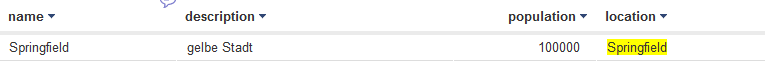
\includegraphics[scale=0.75]{images/geocoding_failed.png}

Diese geocodierten Standorte werden in der Tabelle hinterlegt sind aber mit den SQL API nicht selektierbar. Man müsste also für jede Zeile die man als Resultat erhält die Geocodierung selbst vornehmen, was sich negativ auf die Ladezeit der Karte auswirkt.
Es gibt verschiedene Dienste, welche eine solche Geocodierung von Standortdaten anbieten. Die meisten davon haben aber eine Begrenzung der möglichen Anfragen pro Tag.

\begin{tabular}{|l|l|l|}
\hline 
Anbieter & Anfragen pro Tag & URL \\ 
\hline 
Google Maps Geocoding API & 2500 & https://developers.google.com/maps/documentation/geocoding/?hl=de \\ 
\hline 
Yahoo! PlaceFinder API & 50000 & http://developer.yahoo.com/geo/placefinder/ \\ 
\hline 
MapQuest Geocoding API & keine Begrenzung & http://developer.mapquest.com/web/products/dev-services/geocoding-ws \\ 
\hline 
\end{tabular} 

Wie man sieht erreicht man mit diesen Diensten beim Arbeiten mit grossen Datenmengen schnell die Grenzen.

\subsection{Google Maps API FusionTableLayer}
Google bietet von Haus aus aber bereits eine Fusion Table-Integration im Google Maps API V3 an. Damit ist es möglich Tabellen als eigenständige Layer direkt auf der Karte darzustellen.
Die Möglichkeiten dieser Layer sind noch stark eingeschränkt aber die grundlegenden Funktionalitäten für das Arbeiten mit Geodaten sind bereits vorhanden.

So ist es möglich Abfragen mit WHERE-Conditions einzuschränken oder die Stile des Layers selbst zu bestimmen. Man kann beispielsweise Flächen mit Zeckengebieten je nach Intensität des Befalls anders einfärben.

Ein mächtiges Feature ist zudem die Möglichkeit die Daten der Tabelle direkt als Heatmap darzustellen.

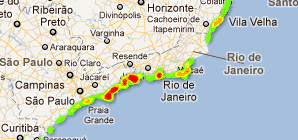
\includegraphics{images/gmap_fusiontableslayer_heatmap.png}

\subsubsection{Vorteil}
Der grösste Vorteil der Fusion Table-Ebenen findet man aber eher darin, dass die Geocodierung der Standort-Daten direkt aus der Tabelle gelesen wird und nicht manuell abgefragt werden muss. Dadurch kann die Ebene komplett auf den Servern von Google aufbereitet werden. Der Client muss die erhaltenen Daten lediglich noch darstellen. Der Vorteil davon wird durch das folgende Diagramm schnell ersichtlich.

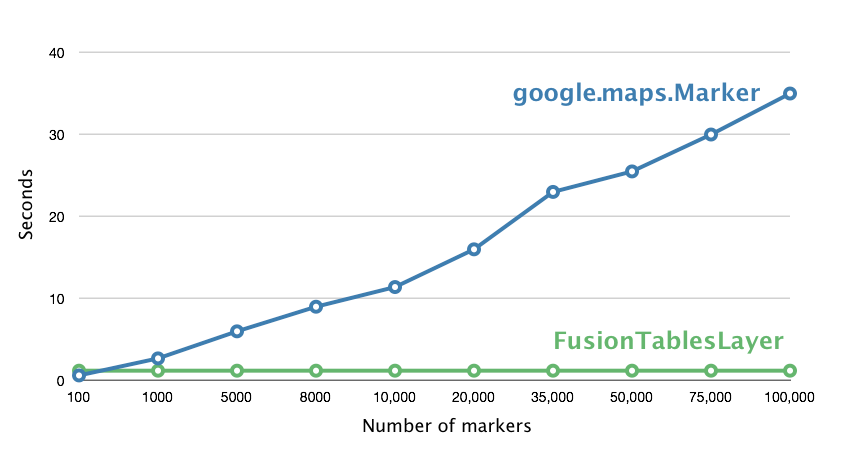
\includegraphics[scale=0.5]{images/gmap_fusiontableslayer_vs_markers.png}

Die Zeit für das Rendering der Karte bleibt demnach beim arbeiten mit Fusion Table-Ebenen konstant und somit unabhängig von der Anzahl Markierungen, welche gesetzt werden müssen. Der Rechenaufwand für das Erstellen der Javascript Marker-Objekte wird direkt von den Google Servern übernommen und das Resultat als Bild zum Client gesendet. Daraus resultiert die konstante Zeit, welche für die Anfrage zum Server und für das Senden der Antwort zum Client verwendet wird.

\subsubsection{Nachteil}
Ein grosser Nachteil dieser Fusion Table-Ebenen besteht aber darin, dass die verwendeten Fusion Tables als  \emph{öffentlich} markiert sein müssen. Sprich jeder kann die Tabellen anzeigen oder auslesen. Es ist also nicht möglich eine Tabelle mit sensiblen Daten als Fusion Table-Ebene darzustellen.

Von Google wird zur Lösung dieses Problems aber folgendes Vorgehen vorgeschlagen: Man kann für Tabellen mit sensiblen Inhalten eine View erstellen, welche lediglich die öffentlichen Spalten und Zeilen selektiert. Diese View könnte man dann als \emph{öffentlich} markieren und in einer Fusion Table-Ebene verwenden.

Es bleibt die Frage offen, wie es möglich ist sensible Daten trotzdem in eine Ebene einzubringen.

\section{Google Fusion Table Javascript Library (gftlib-js)}
Die Google Fusion Table Javascript Library vereinfacht die Kommunikation mit dem Google Fusion Table SQL API. Sie hilft dabei SQL-Queries zu erstellen und per AJAX an das API zu versenden.

Zur Erstellung der AJAX-Requests werden die \$.get()- und \$.post()-Helpermethoden der jQuery Library in der Version 1.7.1 (Minified) verwendet.

\subsection{Methoden}
\begin{tabular}{|l|l|l|}
\hline 
Methode & Beschreibung & Parameter \\ 
\hline 
execSql(callback, query) & Führt einen SQL-Befehl & callback (Funktion): Callback-Methode welche nach Beendigung der Methode aufgerufen wird. query (String): SQL-Query \\ 
\hline 
execSelect(callback, options) & Führt einen SQL-Abfrage aus & callback (Funktion): Callback-Methode welche nach Beendigung der Methode aufgerufen wird. query (String): SQL-Query \\ 
\hline 
convertToObject(gftData) & Konvertiert das Resultat einer Abfrage in sprechende Objekte & • \\ 
\hline 
\end{tabular} 



\section*{Beispiel für Codeschnippsel}
\lstset{language=HTML}
\begin{lstlisting}
<h1>test</h1>
<!-- comment -->
\end{lstlisting}

\section{Überblick}

\section{Vision}

\section{Anforderungsspezifikation}

\section{Analyse}

\section{Design}

\section{Implementation}

\section{Test}

\section{Resultate}

\section{Weiterentwicklung}

\section{Benutzerdokumentation}


% Neue Seite beginnen
\cleardoublepage

% Implementation
% Titel auch in Kopfzeile anzeigen
\markboth{Teil III. Implementation}{Teil III. Implementation}
\part{Implementation}
% Beispielapplikationen
\chapter{Beispielapplikationen}
\label{beispielapplikationen}
Um die verschiedenen Features der Google Fusion Tables kennenzulernen, erstellten wir zu Beginn der Arbeit einige kleine Beispielapplikationen, welche diese verwenden.

Eine Übersicht über alle erstellen Beispiele findet man auf folgender Übersichtsseite: \url{http://gft.rdmr.ch/}

\section{Daten selektieren}
\begin{tabular}{lp{12cm}}
\textbf{URL:} & \url{http://gft.rdmr.ch/examples/js/data-print/} \\ 
\textbf{Zweck:} & Daten mittels gftlib-js von FusionTable selektieren und textuell ausgeben. \\ 
\end{tabular} 

\section{Daten selektieren mit ortsbezogener Einschränkung}
\begin{tabular}{lp{12cm}}
\textbf{URL:} & \url{http://gft.rdmr.ch/examples/js/spatialquery-condition/} \\ 
\textbf{Zweck:} & Daten mittels gftlib-js von FusionTable selektieren und textuell ausgeben. Die Daten werden aber mit dem Spatial-Query \inlinecode{ST\_INTERSECTS} (siehe Abschnitt \ref{sqlapi-spatialqueries}) eingeschränkt. \\ 
\end{tabular} 

\section{Daten selektieren mit ortsbezogener Sortierung}
\begin{tabular}{lp{12cm}}
\textbf{URL:} & \url{http://gft.rdmr.ch/examples/js/spatialquery-order/} \\ 
\textbf{Zweck:} & Daten mittels gftlib-js von FusionTable selektieren und textuell ausgeben. Die zurückgelieferten Daten werden bei der Abfrage mit dem Spatial-Query \inlinecode{ST\_DISTANCE} (siehe Abschnitt \ref{sqlapi-spatialqueries}) sortiert. \\ 
\end{tabular} 

\section{Google Maps: Daten auf Karte anzeigen}
\begin{tabular}{lp{12cm}}
\textbf{URL:} & \url{http://gft.rdmr.ch/examples/js/gmap-rawdata/} \\ 
\textbf{Zweck:} & Daten mittels gftlib-js von FusionTable selektieren und auf Karte anzeigen. \\ 
\end{tabular} 

\section{Google Maps: Daten auf Karte anzeigen mit manueller Geocodierung}
\begin{tabular}{lp{12cm}}
\textbf{URL:} & \url{http://gft.rdmr.ch/examples/js/gmap-geocoding/} \\ 
\textbf{Zweck:} & Daten mittels gftlib-js von FusionTable selektieren und auf Karte anzeigen. Um die Markierungen zu positionieren wird der Geocodierungs-Service des Google Maps API verwendet.  \\ 
\end{tabular} 

\section{Google Maps: Fusion Table-Ebene}
\begin{tabular}{lp{12cm}}
\textbf{URL:} & \url{http://gft.rdmr.ch/examples/js/gmap-fusiontableslayer/} \\ 
\textbf{Zweck:} & Anzeigen der Daten aus zwei FusionTables via FusionTablesLayer.  \\ 
\end{tabular} 

\section{Google Maps: Fusion Table-Ebene Stile}
\begin{tabular}{lp{12cm}}
\textbf{URL:} & \url{http://gft.rdmr.ch/examples/js/gmap-fusiontableslayer-clickstyle/} \\ 
\textbf{Zweck:} & Anzeigen der Daten aus einer FusionTable via FusionTablesLayer mit manuell konfiguriertem Stil (siehe Abschnitt \ref{fusiontableslayer-styles}). Sobald auf eine angezeigte Fläche geklickt wird, ändert sich deren Farbe. \\ 
\end{tabular} 

\section{Google Maps: Dynamische Fusion Table-Ebene}
\begin{tabular}{lp{12cm}}
\textbf{URL:} & \url{http://gft.rdmr.ch/examples/js/gmap-dynamic-fusiontableslayer/} \\ 
\textbf{Zweck:} & Anzeigen der Daten aus zwei FusionTables via FusionTablesLayer. Per Slider lassen sich zusätzlich die zurückgegebenen Daten nach der Anzahl an Einwohnern einschränken.  \\ 
\end{tabular} 

\section{Google Maps: Fusion Table-Ebene mit ortsbezogener Einschränkung}
\begin{tabular}{lp{12cm}}
\textbf{URL:} & \url{http://gft.rdmr.ch/examples/js/gmap-spatialquery/} \\ 
\textbf{Zweck:} & Anzeigen der Daten aus einer FusionTable via FusionTablesLayer. Es werden nur diejenigen Daten angezeigt, welche im Radius der auf der Karte positionierten Markierung liegen. Die Markierung lässt sich per Drag{\&}Drop auf der Karte verschieben. Zusätzlich lässt sich der Radius per Slider definieren. \\ 
\end{tabular} 

\section{Google Charts: Daten mit Diagrammen visualisieren}
\begin{tabular}{lp{12cm}}
\textbf{URL:} & \url{http://gft.rdmr.ch/examples/js/gchart-fusiontable/} \\ 
\textbf{Zweck:} & Visualisieren der Daten aus einer FusionTable mit Diagrammen. Dazu wird das Google Chart Tool API verwendet. \\ 
\end{tabular} 

\section{Einfügen von Daten}
\begin{tabular}{lp{12cm}}
\textbf{URL:} & \url{http://gft.rdmr.ch/examples/js/oauth-login/} \\ 
\textbf{Zweck:} & Einfügen von Daten in eine FusionTable. Dazu muss zuerst ein Zugriffs-Token via OAuth angefordert werden.

\textit{Hinweis: Dieses Beispiel funktioniert nur mit einem Google Account} \\ 
\end{tabular} 

\section{Verwendung einer Fusion Table-Ebene in Sencha Touch 2}
\begin{tabular}{lp{12cm}}
\textbf{URL:} & \url{http://gft.rdmr.ch/examples/js/senchatouch-fusiontableslayer/} \\ 
\textbf{Zweck:} & Anzeige einer FusionTableLayer in einer Sencha Touch 2 Applikation. \\ 
\end{tabular} 

% Use Case 1: WorldData
\chapter{Use Case 1: WorldData}
\label{worlddata}

\section{Einführung}
Im ersten Use Case geht es hauptsächlich um die Anzeige grosser Datenmengen auf der Karte. Dazu importieren wir bestehende Datenbestände in die Google Fusion Tables und visualisieren diese mittels Google Maps API auf der Karte.

\subsection{Ziel}
Es sollen verschiedene historische Länderdaten auf einer Weltkarte angezeigt werden. Die Daten sind pro Jahr und Thema unterteilt. Über eine Zeitachse soll es möglich sein die Daten der verschiedenen Jahre zu selektieren. Eine solche Darstellung kann beispielsweise dabei helfen Zusammenhänge zwischen verschiedenen Themenbereichen zu finden.

\subsection{Vorgehen}
Um die Daten pro Land zu visualisieren, werden zuerst die Landesgrenzen als Geometrie-Datensätze in eine separate Fusion Tabelle importiert. In eine andere Tabelle werden dann die Daten importiert unterteilt nach Land und Jahr. Diese beiden Tabellen werden per Merge-Funktion zu einer Tabelle zusammengefasst, welche dann mittels FusionTablesLayer des Google Maps APIs auf der Karte dargestellt werden kann.

\subsection{Datenquellen}
Als Datenquelle wurde der Daten Katalog der Weltbank\footnote{\url{http://data.worldbank.org/}} verwendet. Darin finden sich länderspezifische Daten aufgeteilt in über 7000 Themenbereiche. Diese lassen sich als XML- oder Excel-Datei herunterladen. Für unseren Import verwendeten wir die Excel-Dateien, welche wir vorbereitet und als CSV-Dateien gespeichert haben. Diese konnten wir als neue Google Fusion Tables importieren.

Die Landesgrenzen wurden als \gls{KML}-Datei von einer inoffiziellen Google Earth Library-Webseite\footnote{\url{http://www.gelib.com/world-borders.htm}} bezogen. 

\section{Analyse}
\todo[inline]{UseCase 1: WorldData - Analyse}

\section{Design}

\subsection{UseCases}

\begin{figure}[H]
	\centering
	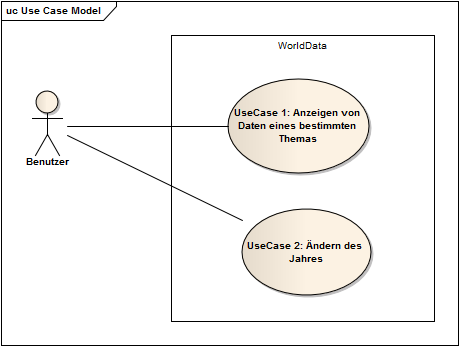
\includegraphics[scale=0.8]{images/usecase1-worlddata/uml/worlddata-usecasemodel.png}
	\caption{WorldData UseCase Modell}
	\label{worlddata-usecasemodel}
\end{figure}

% Use Case 1: Anzeigen von Daten eines bestimmten Themas
\subsubsection{Use Case 1: Anzeigen von Daten eines bestimmten Themas}
\paragraph{Primary Actor}
\begin{itemize}
\item Benutzer
\end{itemize}

\paragraph{Stakeholders and Interests}
\begin{itemize}
\item Benutzer: Möchte Daten zu einem bestimmten Thema auf der Karte anzeigen
\end{itemize}

\paragraph{Preconditions}
\begin{itemize}
\item Webapplikation ist gestartet
\end{itemize}

\paragraph{Success Guarantee (Postconditions)}
\begin{itemize}
\item Daten des gewählten Themas werden auf der Karte angezeigt
\item Legende zu den Daten wird angezeigt
\end{itemize}

\paragraph{Main Success Scenario}
\begin{enumerate}
\item Benutzer wählt das Thema aus
\end{enumerate}

\paragraph{Special Requirements}
-

\paragraph{Frequency of Occurrence}
Tritt sehr häufig auf, da eine beliebige Anzahl von Benutzern die Webapplikation bedienen können.

% Use Case 2: Ändern des Jahres
\subsubsection{Use Case 2: Ändern des Jahres}
\paragraph{Primary Actor}
\begin{itemize}
\item Benutzer
\end{itemize}

\paragraph{Stakeholders and Interests}
\begin{itemize}
\item Benutzer: Möchte Daten eines anderen Jahres anzeigen
\end{itemize}

\paragraph{Preconditions}
\begin{itemize}
\item Webapplikation ist gestartet
\item Thema ist ausgewählt
\end{itemize}

\paragraph{Success Guarantee (Postconditions)}
\begin{itemize}
\item Daten des gewählten Jahres werden auf der Karte angezeigt
\end{itemize}

\paragraph{Main Success Scenario}
\begin{enumerate}
\item Benutzer wählt das gewünschte Jahr aus
\end{enumerate}

\paragraph{Alternative Flows}
1a. Falls für das gewählte Jahr keine Daten vorhanden sind, ist dies ebenfalls auf der Karte ersichtlich.

\paragraph{Special Requirements}
-

\paragraph{Frequency of Occurrence}
Tritt sehr häufig auf, da eine beliebige Anzahl von Benutzern die Webapplikation bedienen können.

\subsection{ERD}
\begin{figure}[H]
	\centering
	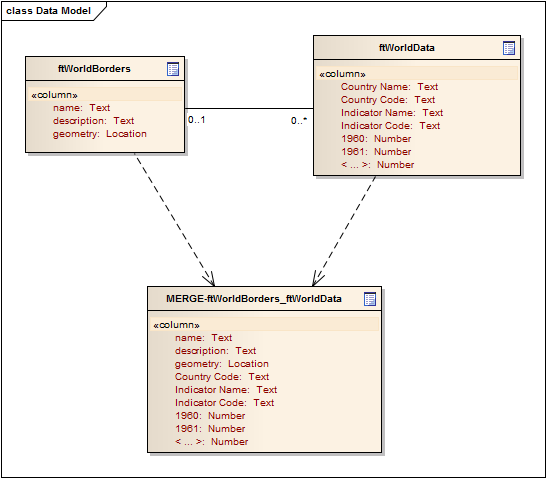
\includegraphics[scale=0.8]{images/usecase1-worlddata/uml/worlddata-erd.png}
	\caption{WorldData ERD}
	\label{worlddata-erd}
\end{figure}

\subsection{Klassendiagramm}
\begin{figure}[H]
	\centering
	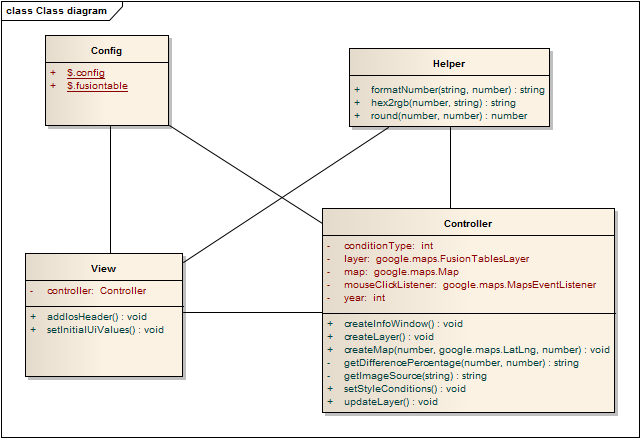
\includegraphics[scale=0.7]{images/usecase1-worlddata/uml/worlddata-classdiagram.png}
	\caption{WorldData Klassendiagramm}
	\label{worlddata-classdiagram}
\end{figure}

\section{Implementation}
Die Applikation wurde als Webapplikation implementiert. Für die GUI-Elemente wurde das Javascript Framework jQuery Mobile verwendet. Dieses bietet eine sehr grosse Plattform-Unterstützung, was im Webbereich sehr wichtig ist.

\subsection{Systemanforderungen:}
Da es sich um eine Webapplikation handelt, ist es möglich die Applikation auf beinahe allen Geräten, welche über einem Browser verfügen zu starten. Einschränkungen gibt es nur in den unterstützten Browsern. Eine Liste davon findet sich auf der Webseite des jQuery Mobile Frameworks:  \url{http://jquerymobile.com/blog/2012/04/06/jquery-mobile-1-1-0-rc2/#platforms}

\subsection{Abhängigkeiten}
\begin{longtable}{|l|l|p{8cm}|}
\hline 
\textbf{Library} & \textbf{Version} & \textbf{Verwendung} \\ 
\hline 
jQuery Mobile & 1.1.0 & GUI-Elemente \\ 
\hline 
jQuery & 1.7.1 & Basis für den Gebrauch von jQuery Mobile \\ 
\hline 
Google Maps API & V3 & Karte mit FusionTablesLayer \\ 
\hline 
Cubiq - Add to home screen & 2.0 & Popup welches auf allen iOS Geräten erscheint \\ 
\hline 
\end{longtable} 

\subsection{Quellcode-Struktur}
\begin{longtable}{|l|p{12.5cm}|}
\hline 
\textbf{Datei} & \textbf{Beschreibung} \\ 
\hline 
images/ & Bilder der Applikation \\ 
\hline 
js/ & JavaScripts der Applikation \\ 
\hline 
js/Config.js & Konfiguration der Applikation \\ 
\hline 
js/Controller.js & Controller der Applikation \\ 
\hline 
js/Helper.js & Helper-Funktionen welche von der Applikation verwendet werden \\ 
\hline 
js/View.js & Steuert die Anzeige der Applikation \\ 
\hline 
lib/ & Von der Applikation verwendete Libraries \\ 
\hline 
styles/ & CSS-Styles der Applikation \\ 
\hline
index.html & Startseite der Applikation \\ 
\hline
\end{longtable} 

\section{Test}
\todo[inline]{UseCase 1: WorldData - Test}

\section{Resultate}
Das FusionTablesLayer Element der Google Maps API eignet sich sehr gut zur Darstellung einer grossen Anzahl von Daten. Leider hindern die Einschränkungen betreffend Styles (siehe Abschnitt  \ref{fusiontableslayer-styles-restrictions}) stark den individuellen Gestalltungsprozess der Ebene.

Wie wir feststellen mussten, sind diese 5 Stile sehr schnell aufgebraucht. Einer davon fällt meistens für den Standard-Stil weg. Dieser wird angewendet, wenn die entsprechende Zeile aus der Tabelle auf keine Bedingung der restlichen Stile passt. So bleiben lediglich noch 4 Stile übrig für alle Elemente die man speziell hervorheben möchte.

Sobald man dann auch noch verschiedene Geometrie-Typen in der Tabelle abgelegt hat (Punkt, Linie, Fläche), muss man sich gut überlegen, für welche Elemente man wirklich einen speziellen Stil anwenden will.

\section{Weiterentwicklung}
Da es sich bei der Applikation lediglich um einen Prototypen handelt, bietet diese natürlich noch ein grosses Potential zur Weiterentwicklung. Hier eine Auflistung möglicher Features, welche noch implementiert werden könnten:

\begin{itemize}
\item Weitere Themen in die Datenbank importieren
\item Auswahl der Länder für welche Daten angezeigt werden sollen
\item Anzeige einer Rangliste der 10 Länder mit den höchsten Werten des gewählten Themas
\item Direkter Vergleich verschiedener Länder
\end{itemize}


\section{Benutzerdokumentation}
\subsection{Importieren der Daten in Google Fusion Tables}

\subsubsection{Landesgrenzen}
\label{landesgrenzen}
Die Landesgrenzen liegen als KML-Datei vor. Diese beinhaltet alle Länder mit ihren Grenzen definiert als Polygone.

\begin{figure}[!h]
	\centering
	
\includegraphics{images/usecase1-worlddata/documentation/worlddata-worldborders_kml.png}
	\caption{WorldData Landesgrenzen liegen als KML-Datei vor}
	\label{worlddata-worldborders_kml}
\end{figure}

\begin{enumerate}
\item Google Drive öffnen (\url{https://drive.google.com/}) und sich mit seinem Google Account einloggen
\item Erstellen > Mehr > Fusion Tabelle (Beta) \\ 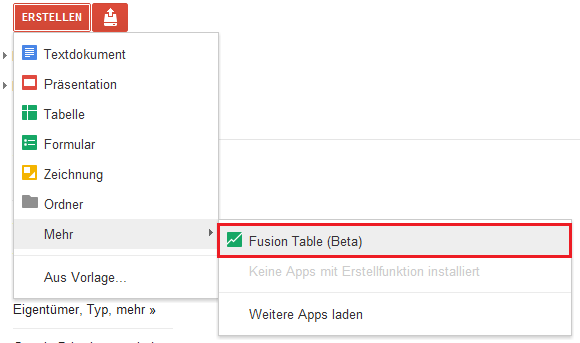
\includegraphics{images/usecase1-worlddata/documentation/worlddata-worldborders_import1.png}
\item Es öffnet sich die neue Fusion Table mit dem Dialog zum Importieren von bestehenden Daten
\item Im Tab \emph{From this computer} die lokal gespeicherte Datei auswählen > Next
\item Die Daten werden automatisch in passende Spalten eingeteilt
\item Abschliessend muss der Tabelle noch einen Namen gegeben werden
\item Mit \emph{Finish} werden die Daten dann importiert
\end{enumerate}

Die Tabelle sollte nun folgendermassen aussehen:

\begin{figure}[H]
	\centering
	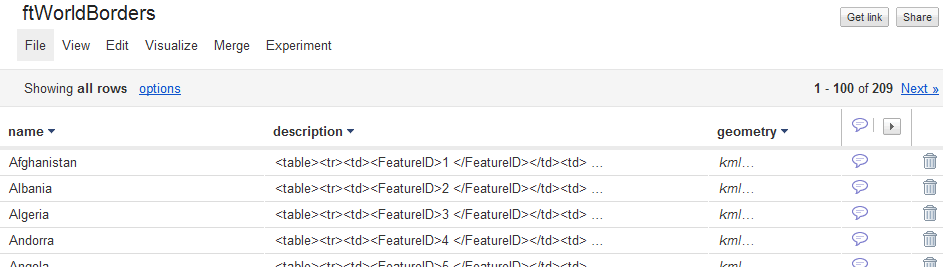
\includegraphics[scale=0.65]{images/usecase1-worlddata/documentation/worlddata-worldborders_import_done.png}
	\caption{WorldData Landesgrenzen erfolgreich als Fusion Table importiert}
	\label{worlddata-worldborders_import_done}
\end{figure}

\subsubsection{Daten}
Die Daten liegen als CSV-Datei vor. Diese beinhaltet folgende Spalten:
\begin{itemize}
\item Country Name
\item Country Code
\item Indicator Name
\item Indicator Code
\item 1960
\item 1961
\item ...
\end{itemize}

\begin{figure}[H]
	\centering
	
\includegraphics{images/usecase1-worlddata/documentation/worlddata-data_csv.png}
	\caption{WorldData Daten liegen als CSV-Datei vor}
	\label{worlddata-data_csv}
\end{figure}

Das Vorgehen für den Import der Daten ist dasselbe wie bei den Landesgrenzen (siehe Abschnitt \ref{landesgrenzen}).

Nach dem Import der Daten sollte die Tabelle folgendermassen aussehen:

\begin{figure}[H]
	\centering
	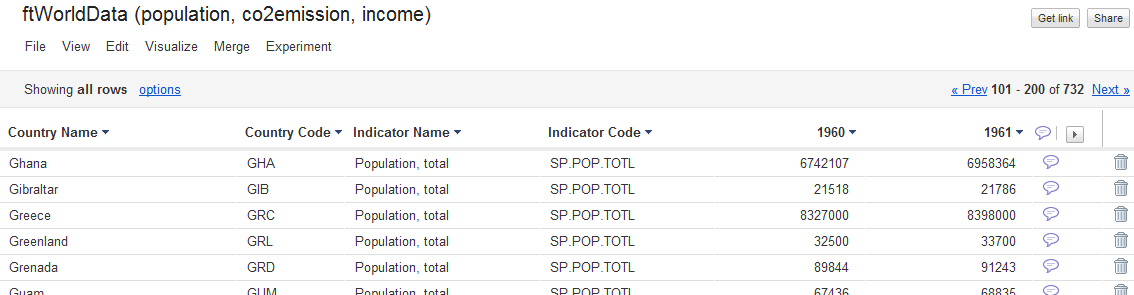
\includegraphics[scale=0.5]{images/usecase1-worlddata/documentation/worlddata-data_import_done.png}
	\caption{WorldData Daten erfolgreich als Fusion Table importiert}
	\label{worlddata-data_import_done}
\end{figure}

\subsubsection{Tabellen mergen}
Sind beide Fusion Tables erstellt müssen diese zusammengefügt werden, um sie schlussendlich als einen einzelnen Layer auf der Karte darzustellen. Dazu bietet Google Fusion Tables die \emph{Merge}-Funktion an. 

\begin{enumerate}
\item Eine der beiden Tabellen öffnen
\item Im Menü \emph{Merge} auswählen \\ 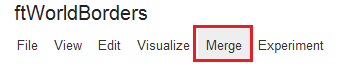
\includegraphics{images/usecase1-worlddata/documentation/worlddata-merge1.png}
\item Es öffnet sich ein Popup, welches durch den Vorgang führt
\item In der 1. Spalte wählt man die Spalte aus, über welche die beiden Tabellen verbunden werden sollen. In unserem Fall ist dies die Spalte mit den Namen der Länder.
\item In der 2. Spalte muss man zuerst die andere Tabelle auswählen und dann ebenfalls die Spalte, in welcher die Namen der Länder gespeichert sind.
\item Schlussendlich muss der neuen Tabelle ein Namen gegeben werden
\item Mit einem Klick auf \emph{Merge tables} wird die neue Tabelle mit den zusammengefügten Daten erstellt. \\ 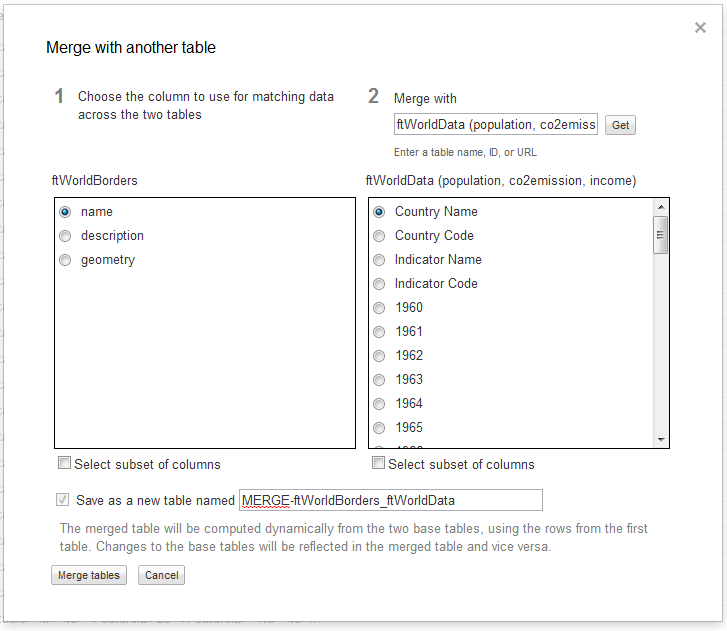
\includegraphics[scale=0.8]{images/usecase1-worlddata/documentation/worlddata-merge2.png}
\end{enumerate}

Die zusammengeführte Tabelle sollte nun folgendermassen aussehen:

\begin{figure}[H]
	\centering
	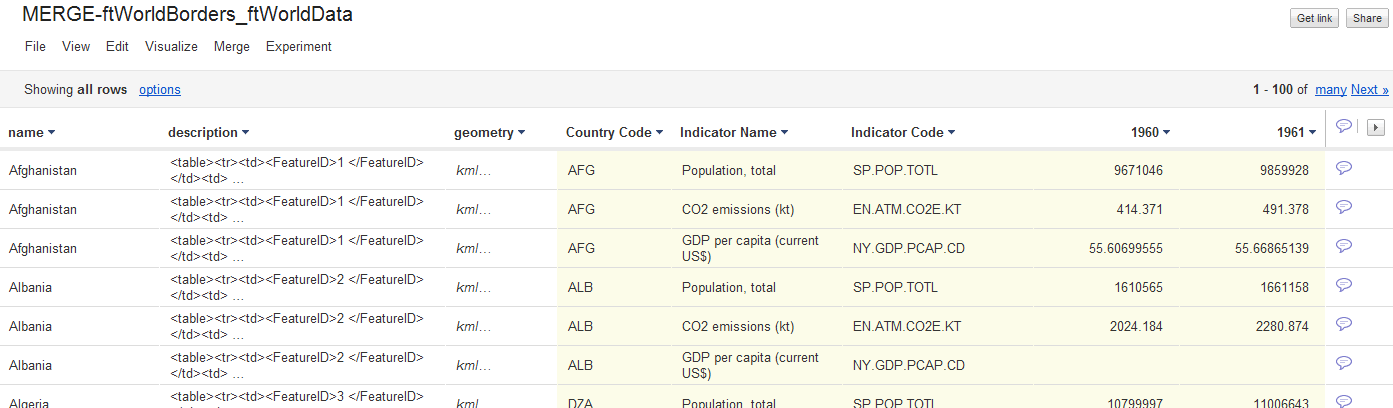
\includegraphics[scale=0.4]{images/usecase1-worlddata/documentation/worlddata-merge_done.png}
	\caption{WorldData Merge der Landesgrenzen- und Daten-Tabelle}
	\label{worlddata-merge_done}
\end{figure}

\subsubsection{Merge-Tabelle für die Verwendung mit FusionTablesLayer vorbereiten}
Um die Tabelle nun als FusionTablesLayer verwenden zu können, muss diese als \emph{öffentlich} markiert werden. Dazu klickt man bei der geöffneten Tabelle auf den \emph{Share}-Button in der linken oberen Ecke.

\begin{figure}[H]
	\centering
	
\includegraphics{images/usecase1-worlddata/documentation/worlddata-prepare_fusiontableslayer1.png}
	\caption{WorldData Freigabe der Merge-Tabelle}
	\label{worlddata-prepare_fusiontableslayer1}
\end{figure}

Im Dialogfenster wählt man unter \emph{Visibility options} den Eintrag \emph{Public} aus.

\begin{figure}[H]
	\centering
	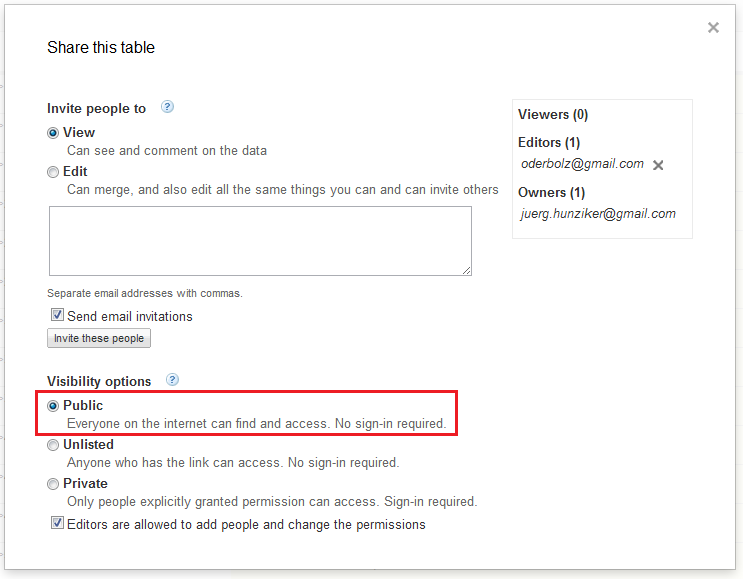
\includegraphics[scale=0.5]{images/usecase1-worlddata/documentation/worlddata-prepare_fusiontableslayer2.png}
	\caption{WorldData Freigabeeinstellungen der Merge-Tabelle}
	\label{worlddata-prepare_fusiontableslayer2}
\end{figure}

Als letzten Schritt muss man sich noch die eindeutige ID der Tabelle merken. Dazu wählt man im Menü  \emph{File > About} und kopiert sich die angezeigte \emph{Encrypted ID} im geöffneten Dialog.

\begin{figure}[H]
	\centering
	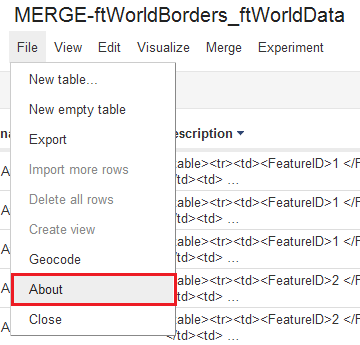
\includegraphics{images/usecase1-worlddata/documentation/worlddata-prepare_fusiontableslayer3.png}
	\caption{WorldData ID der Merge-Tabelle finden}
	\label{worlddata-prepare_fusiontableslayer3}
\end{figure}

\begin{figure}[H]
	\centering
	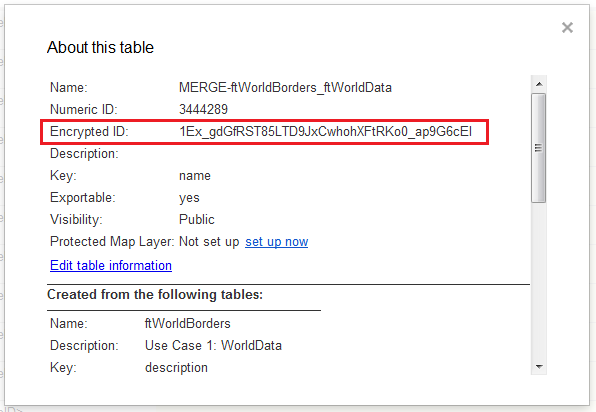
\includegraphics[scale=0.8]{images/usecase1-worlddata/documentation/worlddata-prepare_fusiontableslayer4.png}
	\caption{WorldData ID der Merge-Tabelle Dialog}
	\label{worlddata-prepare_fusiontableslayer4}
\end{figure}

\subsection{Konfiguration der Applikation}
Um die eben erstellte Fusion Table nun in der WorldData-Applikation zu verwenden muss diese folgendermassen konfiguriert werden.

\subsubsection{/js/Config.js}
\begin{longtable}{|l|l|p{8cm}|}
\hline 
\textbf{Parameter} & \textbf{Typ} & \textbf{Beschreibung} \\ 
\hline 
\inlinecode{\$.fusiontable.id} & int & Öffnetliche ID der zu verwendenden Fusion Table \\ 
\hline 
\inlinecode{\$.fusiontable.field} & string & Spaltenname welcher die Landesgrenzen speichert

\textit{(ACHTUNG: Gross-/Kleinschreibung relevant)} \\ 
\hline 
\inlinecode{\$.fusiontable.typeField} & string & Spaltenname aus welchem die Themen gelesen werden sollen

\textit{(ACHTUNG: Gross-/Kleinschreibung relevant)} \\ 
\hline 
\inlinecode{\$.fusiontable.types} & - & Konfiguration der verschiedenen Themen. Für jedes Thema muss ein neuer Block nach folgendem Schema erstellt werden:

\lstset{language=JavaScript}
\begin{lstlisting}
'<TYPE>': {
	name: '<TYPE.name>',
	styleBoundaries: {
		low: <TYPE.styleBoundaries.low>,
		medium: <TYPE.styleBoundaries.medium>,
		high: <TYPE.styleBoundaries.high>
	}
}
\end{lstlisting} \\ 
\hline 
\inlinecode{TYPE} & string & ID des Themas \\ 
\hline 
\inlinecode{TYPE.name} & string & Bezeichnung des Themas \\ 
\hline 
\inlinecode{TYPE.styleBoundaries.low} & int & Obere Grenze für tiefe Werte \\ 
\hline 
\inlinecode{TYPE.styleBoundaries.medium} & int & Obere Grenze für mittlere Werte \\ 
\hline 
\inlinecode{TYPE.styleBoundaries.high} & int & Obere Grenze für hohe Werte \\ 
\hline 
\end{longtable}

\subsection{Starten der Applikation}
Beim Starten der Applikation sollten nun alle Themen der angegebenen Fusion Table in das Auswahlfeld \emph{Ebene auswählen...} geladen werden.

\begin{figure}[H]
	\centering
	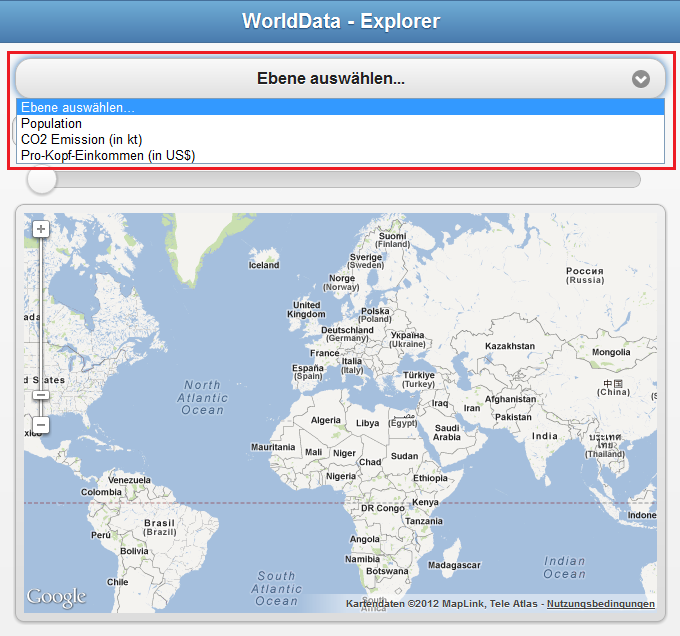
\includegraphics[scale=0.7]{images/usecase1-worlddata/documentation/worlddata-application_start.png}
	\caption{WorldData Auswahlliste der Themen}
	\label{worlddata-application_start}
\end{figure}

% Use Case 2: FixMyStreet
\chapter{Use Case 2: FixMyStreet}
\label{fixmystreet}

\begin{center}

\includegraphics[scale=0.8]{images/usecase2-fixmystreet/fixmystreet-icon_with_gloss}

{\large \textbf{\url{http://fixmystreet.rdmr.ch/}}}
\end{center}

% Einführung
\section{Einführung}
\subsection{Idee}
FixMyStreet ist ein Konzept, welches bereits in verschiedenen Städten bzw. Ländern umgesetzt wurde. Beispiele dafür sind Deutschland welches dazu die Webseite  \url{http://de.seeclickfix.com/} anbietet oder England mit der Webseite \url{http://www.fixmystreet.com/}. Beide Beispiele bieten neben der Webseite auch native Apps für iOS und Android an.

Die Idee hinter dem Konzept ist so einfach wie auch genial. Man ermöglicht dem Bürger per Webseite oder App entdeckte Defekte in seiner Umgebung (defekte Strassenlampen, Schlaglöcher, usw.) direkt der dafür zuständigen Behörde zu melden. Diese kann dann die erhaltenen Meldungen überprüfen und wenn nötig beheben. So können teure Kontrollfahrten auf ein Minimum reduziert werden.

% Ziel
\subsection{Ziel}
Das Ziel dieses Use Cases war die Erstellung einer WebApp, welche genau dieses Konzept umsetzt. Die Benutzer sollen die Möglichkeit haben Defekte in ihrer Umgebung dem zuständigen Amt zu melden.

Google Fusion Table soll dazu als Datenbank verwendet werden, in der die Defekte abgelegt werden. Natürlich sollen auch einige GIS-Features der Fusion Table verwendet werden, um beispielsweise nur die Defekte im aktuell sichtbaren Bereich der Karte zu laden.

% Analyse
\section{Analyse}

\subsection{Storyboard}
Zur Visualisierung der FixMyStreet-Idee wurde vorausgehend ein Storyboard erstellt.

\begin{enumerate}
\item Claudia entdeckt auf ihrem Heimweg eine defekte Strassenlampe \\ 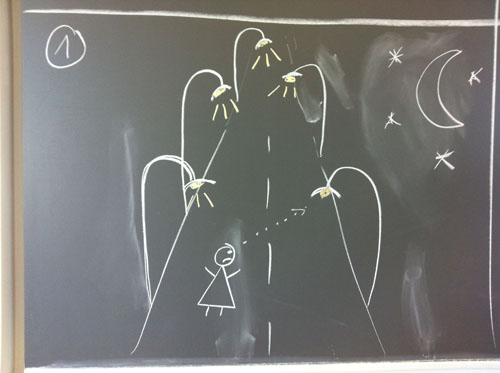
\includegraphics[scale=0.4]{images/usecase2-fixmystreet/storyboard/fixmystreet-storyboard-1.jpg}
\item Sie öffnet die \emph{Fix my street}-App auf ihrem Handy und meldet den Standort der defekten Strassenlampe \\ 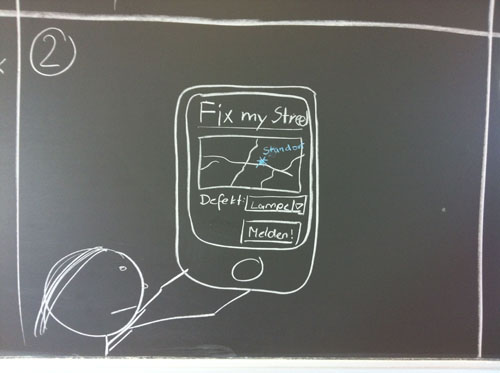
\includegraphics[scale=0.4]{images/usecase2-fixmystreet/storyboard/fixmystreet-storyboard-2.jpg}
\item Am nächsten Tag überprüft der Werkshofleiter Franz die neuen gemeldeten Fälle im System und findet den Eintrag von Claudia \\ 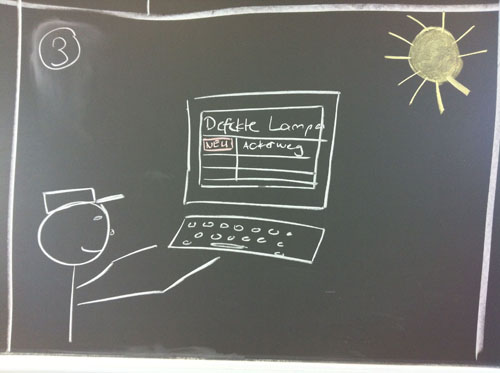
\includegraphics[scale=0.4]{images/usecase2-fixmystreet/storyboard/fixmystreet-storyboard-3.jpg}
\item Er macht sich auf den Weg und repariert die defekte Strassenlampe welche Claudia gemeldet hat \\ 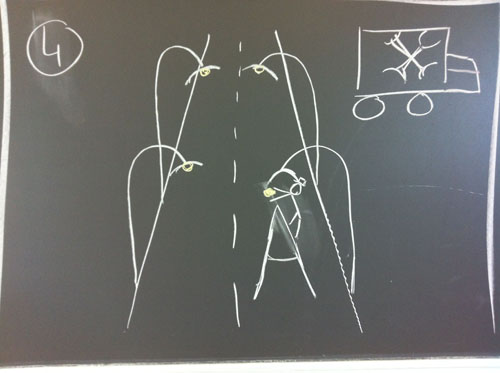
\includegraphics[scale=0.4]{images/usecase2-fixmystreet/storyboard/fixmystreet-storyboard-4.jpg}
\item Am Abend darauf stellt Claudia erfreut fest, dass die Strassenlampe bereits repariert wurde \\ 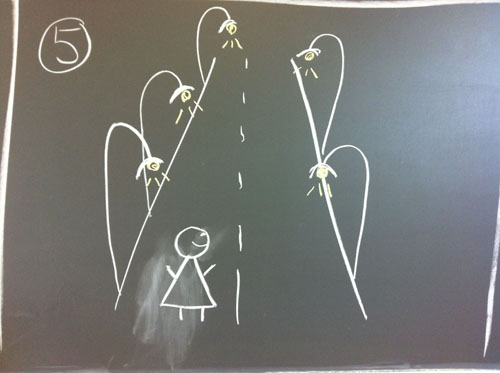
\includegraphics[scale=0.4]{images/usecase2-fixmystreet/storyboard/fixmystreet-storyboard-5.jpg}
\end{enumerate}

\subsection{Use Cases}
Die \emph{FixMyStreet}-WebApp soll folgende Use Cases abdecken.

\begin{figure}[H]
	\centering
	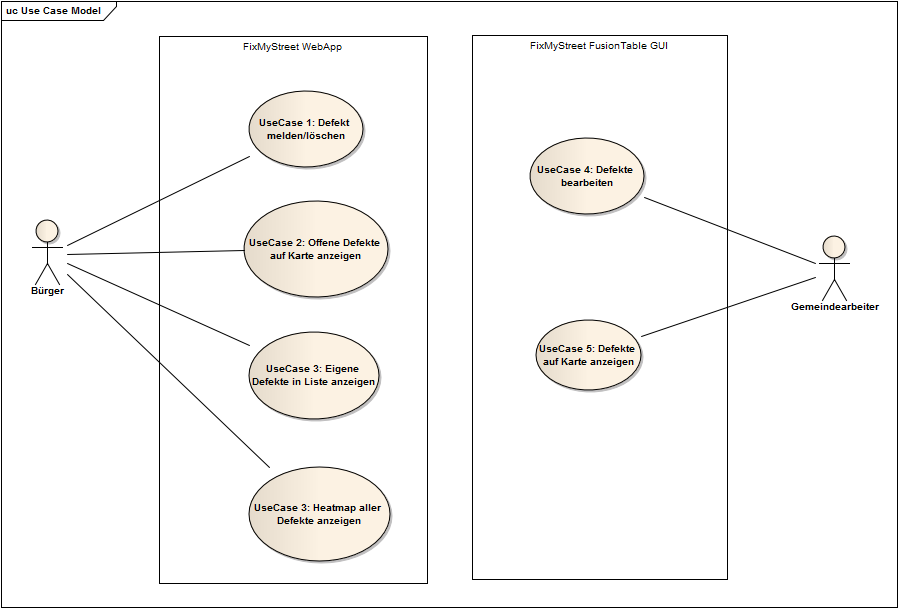
\includegraphics[width=\textwidth]{images/usecase2-fixmystreet/uml/fixmystreet-usecasemodel}
	\caption{FixMyStreet: UseCase Modell}
	\label{fixmystreet-usecasemodel}
\end{figure}

% Use Case 1a: Defekt melden
\subsubsection{Use Case 1a: Defekt melden}
\paragraph{Primary Actor}
\begin{itemize}
\item Bürger
\end{itemize}

\paragraph{Stakeholders and Interests}
\begin{itemize}
\item Bürger: Möchte einen entdeckten Defekt melden
\end{itemize}

\paragraph{Preconditions}
\begin{itemize}
\item WebApp ist gestartet
\end{itemize}

\paragraph{Success Guarantee (Postconditions)}
\begin{itemize}
\item Neuer Defekt ist in Datenbank gespeichert
\item Defekt ist in der Liste und auf der Karte ersichtlich
\item Melde-Maske wurde in den Ursprungszustand zurückgesetzt (kein Defekttyp ausgewählt, Markierung wieder auf die aktuelle Position verschoben)
\end{itemize}

\paragraph{Main Success Scenario}
\begin{enumerate}
\item Bürger wählt Defekttypen aus
\item Bürger verschiebt Markierung auf Karte zur Position des Defekts
\item Bürger sendet den Defekt ab
\item Bürger bestätigt die Kontrollfrage, ob der defekt tatsächlich gesendet werden soll
\end{enumerate}

\paragraph{Alternative Flows}
2a. Markierung muss nicht zwangsläufig verschoben werden. Sie zeigt beim Starten der WebApp auf die aktuelle Position. Falls dies nicht zugelassen wird zeigt sie auf einen vorkonfigurierten Ort.

\paragraph{Special Requirements}
-

\paragraph{Frequency of Occurrence}
Tritt sehr häufig auf, da eine beliebige Anzahl von Bürgern Defekte melden kann.

% Use Case 1b: Defekt löschen
\subsubsection{Use Case 1b: Defekt löschen}
\paragraph{Primary Actor}
\begin{itemize}
\item Bürger
\end{itemize}

\paragraph{Stakeholders and Interests}
\begin{itemize}
\item Bürger: Möchte einen bereits gemeldeten Defekt löschen
\end{itemize}

\paragraph{Preconditions}
\begin{itemize}
\item WebApp ist gestartet
\item Die Listenansicht wurde geöffnet 
\item Es wurde bereits ein Defekt gemeldet
\end{itemize}

\paragraph{Success Guarantee (Postconditions)}
\begin{itemize}
\item Der Defekt wurde aus der Datenbank gelöscht
\item Defekt ist nicht mehr auf der Liste und auf der Karte ersichtlich
\end{itemize}

\paragraph{Main Success Scenario}
\begin{enumerate}
\item Bürger markiert den zu löschenden Defekt in der Liste
\item Bürger wählt den Befehl \emph{Löschen}
\end{enumerate}

\paragraph{Alternative Flows}
2a. Falls der Status des Defektes bereits von einem Gemeindearbeiter geändert wurde (in beispielsweise \emph{In Bearbeitung} oder in \emph{Erledigt}, ist es für den Bürger nicht mehr möglich den Defekt zu löschen.

\paragraph{Special Requirements}
-

\paragraph{Frequency of Occurrence}
Tritt sehr häuft auf, da es für jeden Bürger, welcher bereits einen Defekt gemeldet hat, möglich ist seine eigenen Defekte wieder zu löschen.

% Use Case 2: Noch nicht behobene Defekte auf Karte anzeigen
\subsubsection{Use Case 2: Noch nicht behobene Defekte auf Karte anzeigen}
Der Bürger öffnet die Übersicht. Darin werden ihm alle noch nicht behobene Defekte grafisch auf der Karte angezeigt. Die Daten werden laufend aktualisiert, damit er immer einen aktuellen Stand der Defekte sieht.

% Use Case 3: Heatmap aller Defekte anzeigen
\subsubsection{Use Case 3: Heatmap aller Defekte anzeigen}
Der Bürger öffnet wiederum die Übersicht. Darin hat er die Möglichkeit die Defekte als Heatmap darstellen zu lassen. Dabei werden ihm Gebiete in denen viele Defekte gemeldet wurden farblich stärker markiert als Gebiete in denen kaum Defekte gemeldet wurden. Diese Ansicht wird ebenfalls laufend aktualisiert. 

% Use Case 4: Defekte bearbeiten
\subsubsection{Use Case 4: Defekte bearbeiten}
Der Gemeindearbeiter öffnet die FixMyStreet Google Fusion Table. Darin findet er eine Liste mit allen gemeldeten Defekten. Diese kann er direkt bearbeiten.

\emph{Hinweis: Dieser Use Case wird vom gegebenen Google Fusion Tables Web-GUI abgedeckt und wird nicht in der FixMyStreet-App realisiert.}

% Use Case 5: Defekte auf Karte anzeigen
\subsubsection{Use Case 5: Defekte auf Karte anzeigen}
Der Gemeindearbeiter öffnet die FixMyStreet Google Fusion Table. Er hat darin die Möglichkeit alle Defekte auf der Karte anzuzeigen.

\emph{Hinweis: Dieser Use Case wird vom gegebenen Google Fusion Tables Web-GUI abgedeckt und wird nicht in der FixMyStreet-App realisiert.}

\subsection{Paper-Prototype}
Vor der Implementation der Oberfläche wurde ein Paper-Prototype des GUI-Design erstellt. Dieses wurde von verschiedenen Personen getestet. Der Prototype besteht aus drei verschiedenen Hauptmasken.

\paragraph{Maske: Melden}
Auf dieser Maske können Defekte gemeldet werden. Dazu lässt sich zuerst der Defekt-Typ wählen. Danach kann man auf der Karte den Standort des Defekts auswählen indem man die Defekt-Markierung darauf verschiebt. Abschliessend lässt sich die Meldung absenden.

\begin{figure}[H]
\subfigure[Defekt melden - Übersicht]{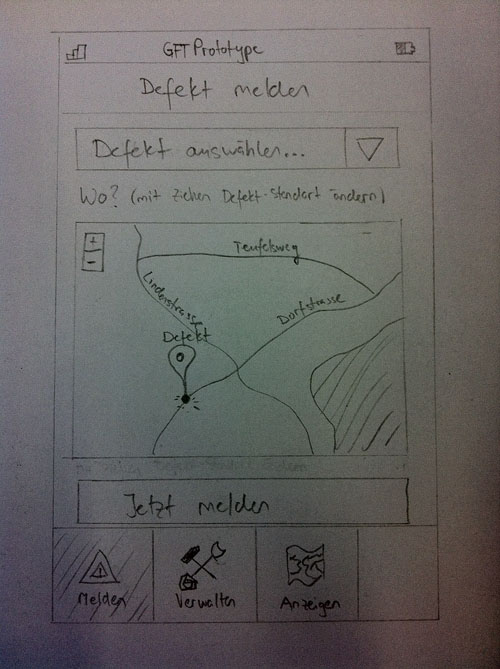
\includegraphics[width=0.45\textwidth]{images/usecase2-fixmystreet/paperprototype/fixmystreet-pp-melden.jpg}}
\hfill
\subfigure[Fehleranzeige beim Absenden ohne Defekttyp-Auswahl]{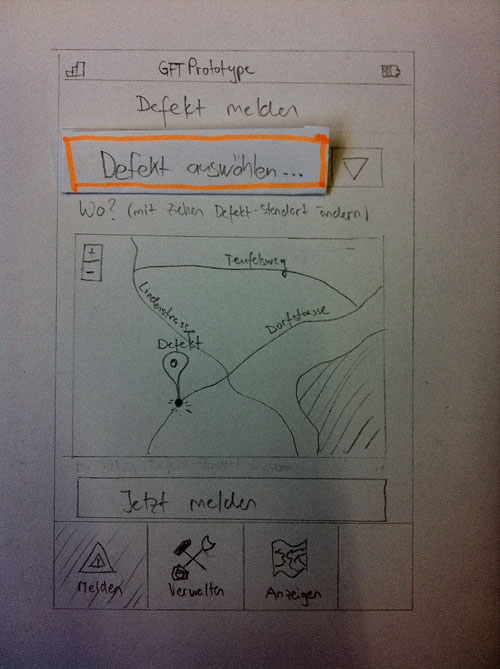
\includegraphics[width=0.45\textwidth]{images/usecase2-fixmystreet/paperprototype/fixmystreet-pp-melden_fehler.jpg}}
\end{figure}

\begin{figure}[H]
\subfigure[Defekttyp-Auswahl aufgeklappt]{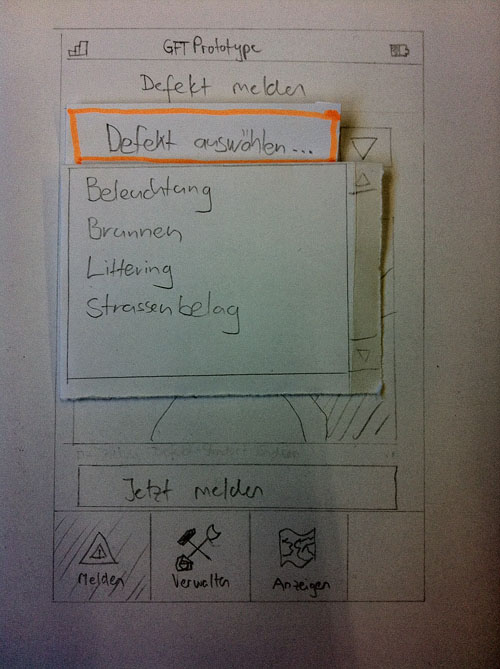
\includegraphics[width=0.45\textwidth]{images/usecase2-fixmystreet/paperprototype/fixmystreet-pp-melden_defektauswaehlen.jpg}}
\hfill
\subfigure[Defekttyp ausgewählt]{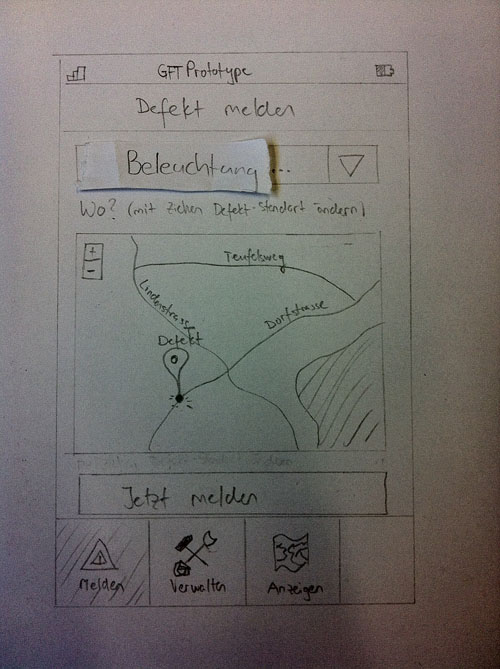
\includegraphics[width=0.45\textwidth]{images/usecase2-fixmystreet/paperprototype/fixmystreet-pp-melden_defektausgewaehlt.jpg}}
\end{figure}

\begin{figure}[H]
\subfigure[Defekt-Markierung auf Karte verschoben]{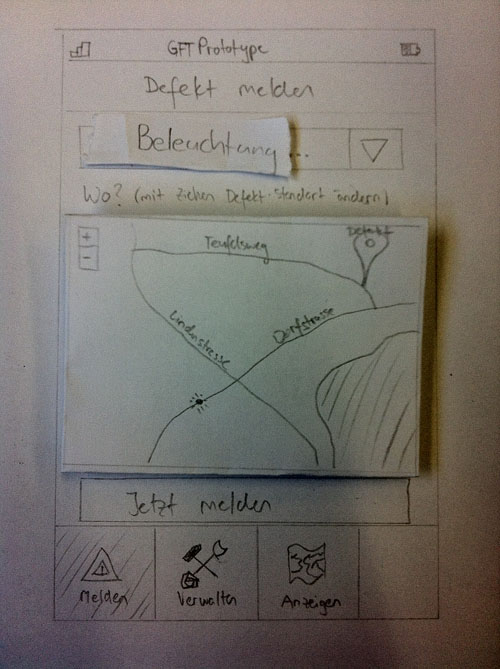
\includegraphics[width=0.45\textwidth]{images/usecase2-fixmystreet/paperprototype/fixmystreet-pp-melden_ortgewaehlt.jpg}}
\hfill
\subfigure[Defekt erfolgreich gemeldet]{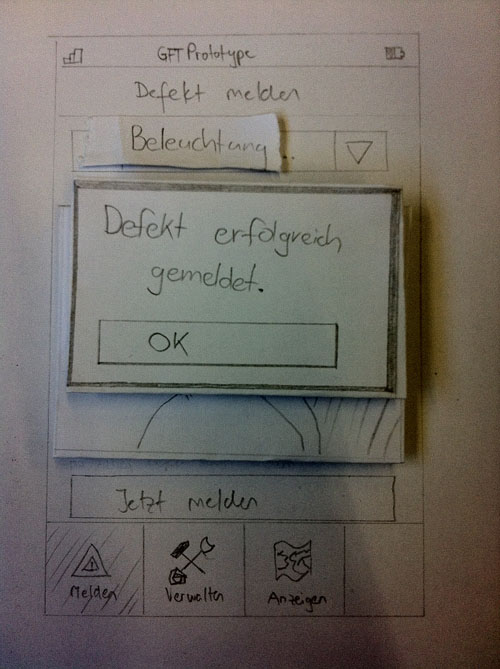
\includegraphics[width=0.45\textwidth]{images/usecase2-fixmystreet/paperprototype/fixmystreet-pp-melden_meldungerfolgreich.jpg}}
\end{figure}

\paragraph{Maske: Verwalten}
In dieser Maske kann man seine eigenen Defekt-Meldungen verwalten. Die gemeldeten Defekte werden gruppiert nach \emph{Offene Defekte} und \emph{Behobene Defekte}. Zu jedem Defekt wird der aktuelle Status angezeigt. Mit einem Klick auf einen Defekt erreicht man dessen Detailanzeige.

\begin{figure}[H]
\subfigure[Defekte verwalten - Übersicht]{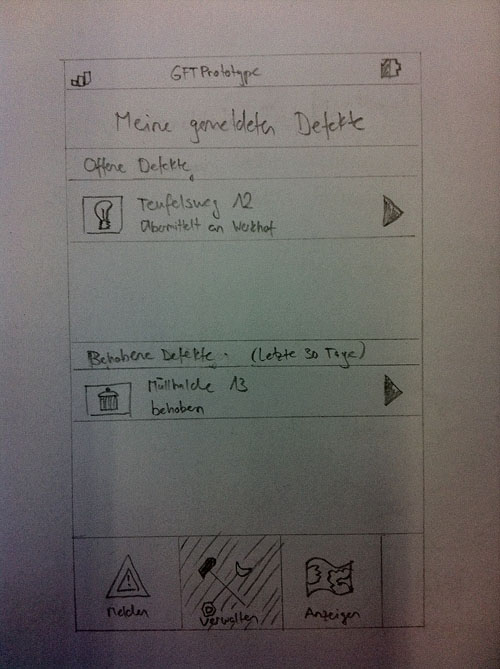
\includegraphics[width=0.45\textwidth]{images/usecase2-fixmystreet/paperprototype/fixmystreet-pp-verwalten.jpg}}
\hfill
\subfigure[Detailansicht eines gemeldeten Defekts]{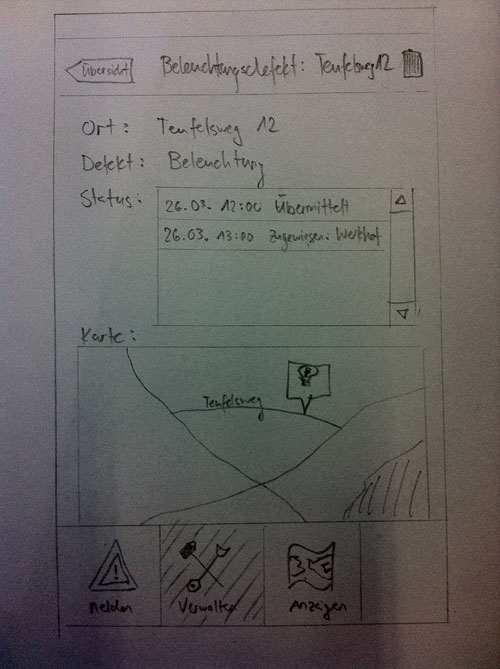
\includegraphics[width=0.45\textwidth]{images/usecase2-fixmystreet/paperprototype/fixmystreet-pp-verwalten_detail.jpg}}
\end{figure}

\paragraph{Maske: Anzeigen}
Auf dieser Maske werden alle gemeldeten Defekte in der Nähe angezeigt. Mit einem Klick auf eine Defekt-Markierung erhält man zusätzliche Information zu diesem Defekt.

\begin{figure}[H]
\subfigure[Anzeigen - Übersicht]{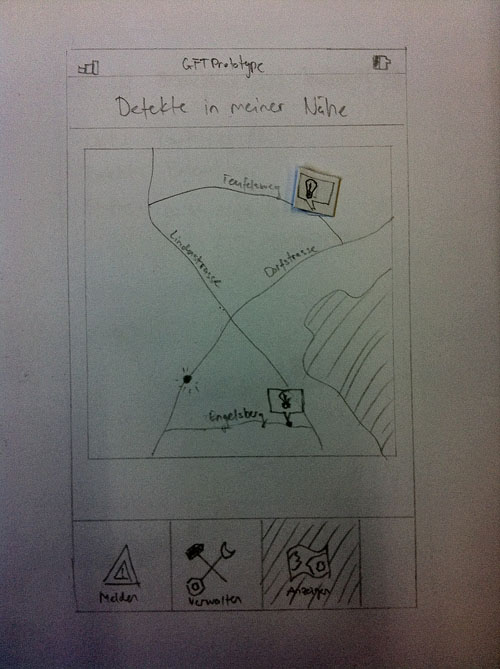
\includegraphics[width=0.45\textwidth]{images/usecase2-fixmystreet/paperprototype/fixmystreet-pp-anzeigen.jpg}}
\end{figure}

% Design
\section{Design}

\subsection{Datenbankschema}
Die Applikation verwendet die FusionTable \emph{ftFixMyStreet}\footnote{\url{https://www.google.com/fusiontables/DataSource?docid=1ggQAh0WF7J7myI27_Pv4anl0wBJQ7ERt4W5E6QQ}}. Davon wurden zwei Views erstellt:

\begin{itemize}
\item \emph{ftFixMyStreet\_Read}\footnote{\url{https://www.google.com/fusiontables/DataSource?docid=1no3_lJ0CCazZVN6rlAY8vrtf9ejoz_xo0e7a9cY}}: In dieser View sind alle gemeldeten Defekte sichtbar, die Applikation hat aber nur Lesezugriff darauf.
\item \emph{ftFixMyStreet\_Write}\footnote{\url{https://www.google.com/fusiontables/DataSource?docid=1EX1S20fZmhetpLuWf_i-Hi5qfx1412a3TbRV1Ac} (private Tabelle)}: In dieser View sind lediglich die Defekte vorhanden deren Status auf \emph{neu} gesetzt ist. Die Applikation kann darin neue Defekte abspeichern und diese auch wieder löschen.
\end{itemize}

\begin{figure}[H]
	\centering
	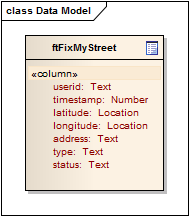
\includegraphics{images/usecase2-fixmystreet/uml/fixmystreet-datamodel}
	\caption{FixMyStreet: Datenbankschema}
	\label{fixmystreet-datamodel}
\end{figure}

\subsection{Klassendiagramm}

\todo[inline]{FixMyStreet: Diagramme beschreiben}

\begin{figure}[H]
	\centering
	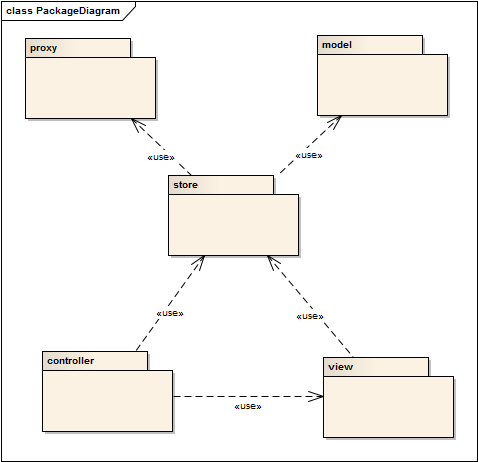
\includegraphics[width=0.8\textwidth]{images/usecase2-fixmystreet/uml/fixmystreet-packagediagram}
	\caption{FixMyStreet: Packagediagramm}
	\label{fixmystreet-packagediagram}
\end{figure}

\begin{figure}[H]
	\centering
	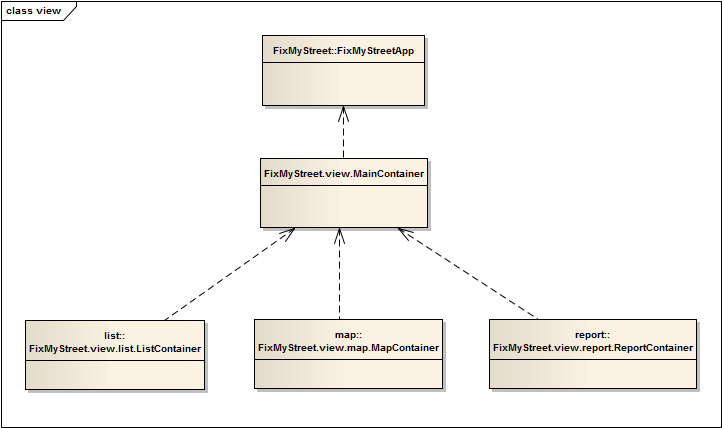
\includegraphics[width=\textwidth]{images/usecase2-fixmystreet/uml/fixmystreet-view-classmodel}
	\caption{FixMyStreet: View Klassendiagramm}
	\label{fixmystreet-view-classmodel}
\end{figure}

\begin{figure}[H]
	\centering
	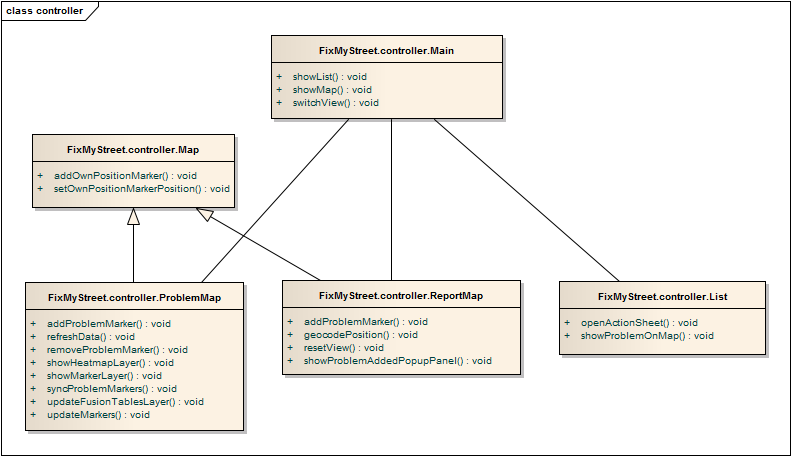
\includegraphics[width=\textwidth]{images/usecase2-fixmystreet/uml/fixmystreet-controller-classmodel}
	\caption{FixMyStreet: Controller Klassendiagramm}
	\label{fixmystreet-controller-classmodel}
\end{figure}

\begin{figure}[H]
	\centering
	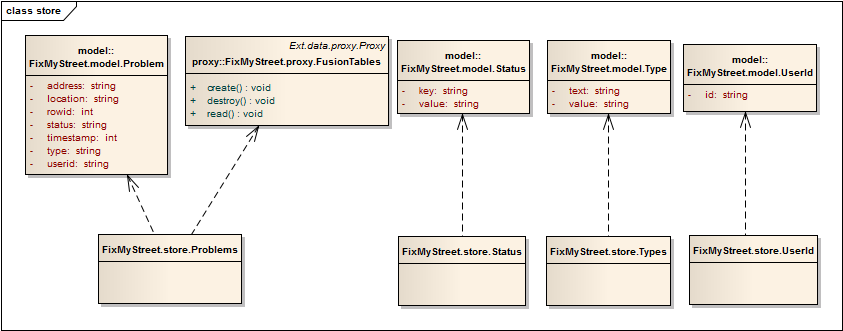
\includegraphics[width=\textwidth]{images/usecase2-fixmystreet/uml/fixmystreet-store-classmodel}
	\caption{FixMyStreet: Stores Klassendiagramm}
	\label{fixmystreet-store-classmodel}
\end{figure}

\subsection{Deploymentdiagramm}
Die Applikation läuft direkt im Browser des Benutzers. Darin greift die \emph{FusionTablesProxy}-Klasse (siehe Abschnitt \ref{fusiontablesproxy}) auf die Fusion Table Client Library \emph{gftlib-js} (siehe Abschnitt \ref{gftlib-js}) zu, welche die Verbindung zur Google Fusion Table erstellt. Dazu wird beim ersten Zugriff ein Zugriffstoken über den \emph{OAuthTokenService} erstellt. Danach kann mit diesem Token auf die Fusion Table \emph{ftFixMyStreet} zugegriffen werden.

\begin{figure}[H]
	\centering
	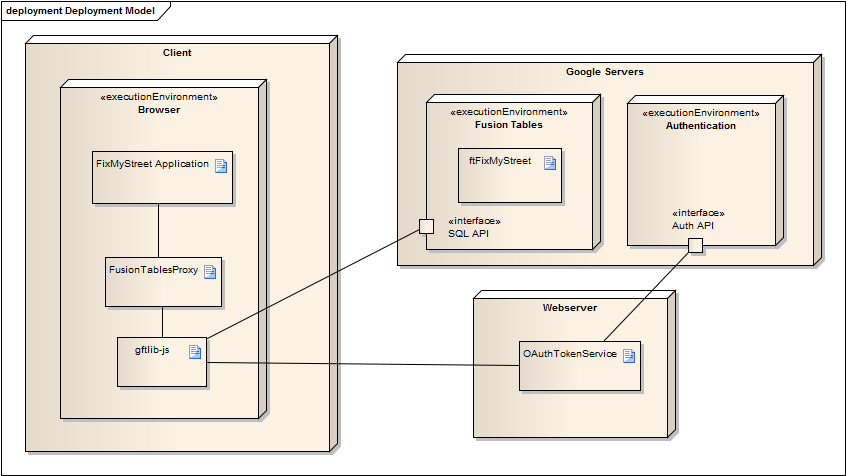
\includegraphics[width=\textwidth]{images/usecase2-fixmystreet/uml/fixmystreet-deploymentmodel}
	\caption{FixMyStreet: Deploymentdiagramm}
	\label{fixmystreet-deploymentmodel}
\end{figure}

\subsection{Starten der Applikation}
Der Benutzer startet die Applikation mit dem Zugriff auf die \emph{index}-Seite, welche die \emph{launch()}-Funktion der Applikation aufruft. Danach werden folgende Schritte durchlaufen:

\begin{enumerate}
\item Laden der verschiedenen Status-Typen
\item Laden der Defekt-Typen
\item Laden der UserId aus dem LocalStorage
\item Falls noch keine UserId vorhanden ist, wird diese generiert und in den LocalStorage geschrieben (siehe Abschnitt \ref{fixmystreet-user-detection})
\item Laden der bereits gemeldeten Defekte des Benutzers aus der Fusion Table
\item Aktueller Standort des Benutzers wird ausgelesen
\item Laden der Benutzeroberfläche
\end{enumerate}

\begin{figure}[H]
	\centering
	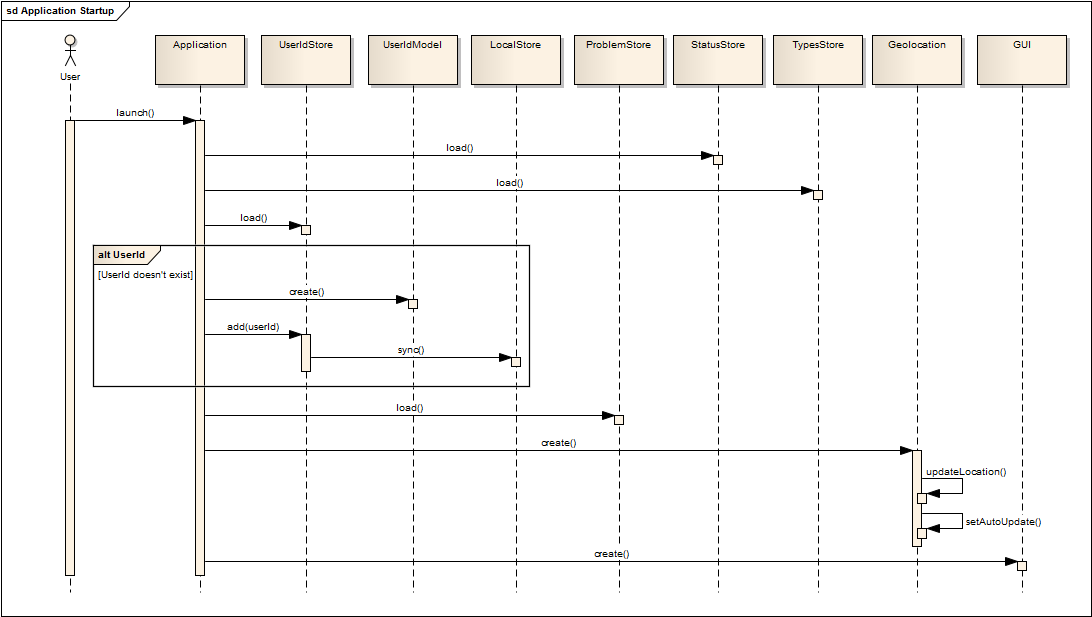
\includegraphics[width=\textwidth]{images/usecase2-fixmystreet/uml/fixmystreet-sequencediagram-applicationstartup}
	\caption{FixMyStreet: Sequenzdiagramm - Starten der Applikation}
	\label{fixmystreet-sequencediagram-applicationstartup}
\end{figure}

% Implementation
\section{Implementation}
Die WebApp basiert auf dem Sencha Touch 2 Framework\footnote{\url{http://www.sencha.com/products/touch/}}. Dieses bietet eine Basis zur Erstellung von mobilen WebApps mit JavaScript.

Das Framework bietet die Möglichkeit eine Applikation streng nach dem MVC-Pattern aufzubauen.

Dazu verwendet Sencha Touch unter anderem das Konzept der Component-Queries\footnote{\url{http://docs.sencha.com/touch/2-0/\#!/api/Ext.ComponentQuery}}. Damit lassen sich View-Komponenten über verschiedene Attribute referenzieren. So kann man beispielsweise über deren eindeutige ID eine Referenz auf das Objekt erstellen.

In den Controller-Klassen werden genau über dieses Konzept Referenzen auf die View-Objekte erstellt und darauf zugegriffen. Damit ist es in fast allen Fällen möglich, die View-Klassen frei von Bussinesslogik zu halten.

\paragraph{Beispiel einer ComponentQuery}
Das folgende Beispiel\footnote{Quelle: \url{http://docs.sencha.com/touch/2-0/\#!/api/Ext.app.Controller} (Stand: 24.05.2012)} zeigt einen Teil eines Controllers. Dieser referenziert im Property \emph{nav} via ComponentQuery die View-Komponente mit der ID \emph{mainNav}.

\lstset{language=JavaScript}
\begin{lstlisting}
Ext.define('MyApp.controller.Main', {
	extend: 'Ext.app.Controller',
	
	config: {
		refs: {
			nav: '#mainNav'
		}
	}
	
	...
});
\end{lstlisting}

\subsection{Systemanforderungen}
Das Sencha Touch 2 Framework unterstützt alle WebKit-fähigen Browser:

\paragraph{Desktop:}
\begin{itemize}
\item Chrome
\item Opera
\item Safari
\end{itemize}

\paragraph{Mobile:}
\begin{itemize}
\item iOS
\item Android
\item Blackberry
\end{itemize}

\subsection{Abhängigkeiten}
\begin{longtable}{|p{0.25\threecelltabwidth}|p{0.1\threecelltabwidth}|p{0.65\threecelltabwidth}|}
\hline 
\textbf{Library} & \textbf{Version} & \textbf{Verwendung} \\ 
\hline 
Sencha Touch 2 & 2.0.1 & Mobile Framework (MVC Applikation) \\ 
\hline 
gftlib-js & 1.0 & Zur Kommunikation mit dem Fusion Table SQL API \\ 
\hline 
jQuery & 1.7.1 & Wird von der gftlib-js verwendet \\ 
\hline 
Google Maps API & V3 & Anzeige der Karten \\ 
\hline 
\caption{FixMyStreet: Abhängigkeiten}
\end{longtable} 

\subsection{Quellcode-Struktur}

\begin{longtable}{|p{0.4\twocelltabwidth}|p{0.6\twocelltabwidth}|}
\hline 
\textbf{Datei} & \textbf{Beschreibung} \\ 
\hline 
\inlinecode{app/app.js} & Startet die Applikation \\ 
\hline 
\inlinecode{app/controller/List.js} & Controller der \emph{List}-View \\ 
\hline 
\inlinecode{app/controller/Main.js} & Haupt-Controller der Applikation (Steuert die einzelnen Ansichten) \\ 
\hline 
\inlinecode{app/controller/Map.js} & Basis-Controller der \emph{Report}-View und der \emph{Map}-View \\ 
\hline 
\inlinecode{app/controller/ProblemMap.js} & Controller der \emph{Map}-View \\ 
\hline 
\inlinecode{app/controller/ReportMap.js} & Controller der \emph{Report}-View \\ 
\hline 
\inlinecode{app/model/*.js} & Daten-Modelle der Applikation (Defekt, Status, ...) \\ 
\hline 
\inlinecode{app/plugin/PullRefresh.js} & PullRefresh Plugin der Liste \\ 
\hline 
\inlinecode{app/proxy/FusionTables.js} & Proxy zur Anbindung der Google Fusion Tabelle an die Applikation \\ 
\hline 
\inlinecode{app/store/*.js} & Daten-Speicher der Applikation (Defekte, Typen, ...) \\ 
\hline 
\inlinecode{app/utli/Config.js} & Konfiguration der Applikation \\ 
\hline 
\inlinecode{app/util/Geolocation.js} & Steuert Zugriff auf aktuelle Geolocation des Geräts \\ 
\hline 
\inlinecode{app/view/*.js} & Views der Applikation \\ 
\hline 
\inlinecode{resources/images/} & Bilder der Applikation \\ 
\hline 
\inlinecode{resources/styles/} & CSS-Styles der Applikation \\ 
\hline 
\inlinecode{index.html} & Einstiegspunkt der Applikation (Inkludiert \inlinecode{app/app.js}, welches die Applikation startet) \\ 
\hline
\caption{FixMyStreet: Quellcode-Struktur}
\end{longtable} 

\subsection{Anbindung an Google Fusion Table}
\label{fusiontablesproxy}
Sencha Touch verwendet für den Zugriff auf fremde Datenquellen das Konzept der Proxies. Ein Proxy verbindet einen internen Applikations-Store mit der eigentlichen Datenquelle.

Es gibt bereits vorgefertigte Proxies, welche die meisten Anwendungsfälle abdecken. So ist es möglich über einen LocalStorage-Proxy mit dem internen Browserspeicher (LocalStorage) zu kommunizieren. Zudem existieren Proxies für AJAX-Serveranfragen oder JSONP-Anfragen.

Für den Zugriff auf die Fusion Table als Datenbank mussten wir aber einen eigenen Proxy schreiben. Dieser verwendet unsere selbst geschriebene JavaScript Fusion Table Library \emph{GftLib} (siehe Abschnitt \ref{gftlib-js}), um über das SQL API mit der Fusion Table zu kommunizieren.
Der Proxy implementiert lediglich die in unserem UseCase verwendeten CRUD-Operationen Create, Read und Delete. Ein Änderung von gemeldeten Defekten ist über die WebApp nicht vorgesehen und wurde deshalb auch nicht implementiert.
Die Operationen sind jeweils in den Methoden \inlinecode{create()}, \inlinecode{read()} und \inlinecode{destory()} des Proxies abgebildet.

\begin{figure}[H]
	\centering
	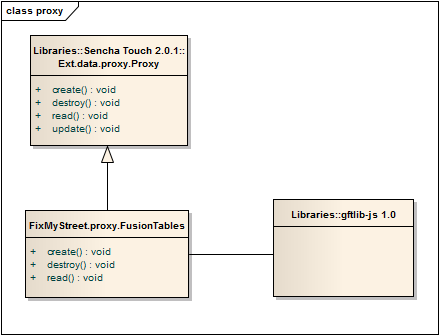
\includegraphics[width=0.7\textwidth]{images/usecase2-fixmystreet/uml/fixmystreet-proxy-classmodel}
	\caption{FixMyStreet: FusionTablesLayer Proxy}
	\label{fixmystreet-proxy-classmodel}
\end{figure}

\subsection{Wiedererkennung des Benutzers}
\label{fixmystreet-user-detection}
Um die Hemmschwelle zur Benutzung der App möglichst klein zu halten, wollten wir möglichst darauf verzichten, dass sich die Benutzer zuerst Registrieren müssen um die App zu verwenden. Trotzdem soll die App die Möglichkeit haben einen Benutzer wiederzuerkennen, um ihm seine bereits gemeldeten Defekte anzeigen zu können.

Wir generieren dazu beim ersten Starten der App eine Version 1 UUID\footnote{\url{http://de.wikipedia.org/wiki/Universally_Unique_Identifier}} (sequenziell) gemäss RFC 4122\footnote{\url{http://tools.ietf.org/html/rfc4122}}. Diese legen wir im LocalStorage des Browsers ab. Die gemeldeten Defekte beinhalten dann jeweils die UUID und können so den Benutzern zugewiesen werden.

Ein Problem ergibt sich aber aus dieser Vorgehensart. Sobald ein Benutzer seinen Browsercache leert oder die App an einem anderen Gerät startet, erhält er eine neue UUID, welche den neu erfassten Defekten zugeordnet wird. So können verwaiste Datensätze in der Datenbank entstehen, welche keinem Benutzer mehr zugeordnet werden können. In unserem Anwendungsfall ist dies aber nicht weiter schlimm, da die gemeldeten Fälle von der zuständigen Behörde direkt via Fusion Tables GUI bearbeitet werden. Darin spielt die Benutzerzuordnung keine Rolle.

\subsection{Automatisches Aktualisieren der Übersichtsmaske}
\label{fixmystreet-polling}
Eine weitere Anforderung war es eine möglichst aktuelle Ansicht aller gemeldeten Fälle zu bieten. Wir haben dazu in der Übersichtsmaske ein Polling implementiert. Dieses aktualisiert alle 30 Sekunden die Markierungen auf der Karte indem es eine Anfrage an die Fusion Table sendet. Gelöschte und erledigte Defekte werden entfernt und Neue hinzugefügt.

Die Karte aktualisiert sich zudem jedes Mal, wenn die Übersichtsmaske aufgerufen wird.

\subsection{Auf Übersichtsmaske nur Defekte im sichtbaren Bereich laden}
Um nicht zu viele Markierungen gleichzeitig zu laden, was sich negativ auf die Performance der Applikation auswirken würde, laden wir auf der Übersichtsmaske nur diejenigen Defekte, welche im aktuell sichtbaren Bereich der Karte liegen. Sobald die Karte verschoben wird oder der Zoom verändert wird, werden die Defekte für den neuen Bereich nachgeladen.

Dazu haben wir vorerst das Spatial-Query \inlinecode{ST\_INTERSECTS} des SQL APIs (siehe Abschnitt \ref{sqlapi-spatialqueries}) verwendet. Als Grenze geben wir diesem als Parameter ein Rechteck bestehend aus zwei Ecken der momentan angezeigten Karte mit.

Aufgrund der Einschränkung, dass neue Datensätze nicht geokodiert werden (siehe Abschnitt \ref{geocodierung-bug}), mussten wir in der letzen Version der Applikation das Spatial-Query wieder entfernen und durch eine eigene \inlinecode{WHERE}-Bedingung ersetzen. Ansonsten würden neu gemeldete Defekte solange nicht auf der Karte angezeigt, bis die Datensätze über das Fusion Tables Web-GUI manuell geokodiert werden.

\subsection{Heatmap-Ansicht auf Übersichtsmaske}
Auf der Übersichtsmaske hat man die Möglichkeit alle gemeldeten Defekte als Heatmap darzustellen. Dazu haben wir das eine Fusion Table-Ebene über die Karte gelegt und dessen Heatmap-Feature (siehe Abschnitt \ref{fusiontableslayer-heatmap}) verwendet. 

\section{Test}
\todo[inline]{FixMyStreet: Tests beschreiben}

\section{Resultate}
Wir hatten einige Probleme bei der Verwendung einer Fusion Table als Datenbank der Applikation. Ein Hauptproblem war klar das Fehlen eines \inlinecode{GRANT}-Mechanismus, wie man ihn von vielen anderen Datenbanksystemen kennt. Die gegebenen Möglichkeiten für die Vergabe von Lese- oder Schreibmöglichkeiten würden für den Gebrauch in einer produktiven Applikation kaum ausreichen.

Zusätzlich konnten wir die GIS-Features, welche Google Fusion Tables anbieten nur minimal nutzen. So hinderte uns die fehlende  Geocodierung von neu eingefügten Datensätzen daran Spatial-Queries zu verwenden (siehe Abschnitt \ref{geocodierung-bug}).

Zudem haben wir bewusst auf die Verwendung einer Fusion Tables-Ebene (siehe Abschnitt \ref{gmap-api-fusiontableslayer}) für die Übersichtsmaske verzichtet, da wir dadurch die Möglichkeit verloren hätten Custom-Markers auf der Karte hinzuzufügen. Dies hätte die Usability der App stark verschlechtert, da man nicht mehr direkt den Typen des markierten Defekts erkannt hätte.

Alles in allem waren die Nachteile bei der Verwendung von Google Fusion Tables als Datenbank wahrscheinlich grösser als deren Vorteile.

\section{Weiterentwicklung}
Auch dieser Use Case hat noch ein grosses Ausbaupotential. So wäre es beispielsweise sinnvoll, wenn man bei der Meldung des Defekts noch ein Foto hinzufügen könnte. Damit könnte man noch genauer zeigen, was wirklich defekt ist. Zudem würde es auch der zuständigen Behörde einfacher fallen Spassmeldungen von echten Defekten zu unterscheiden. Zusätzlich wäre es hilfreich, wenn man die Möglichkeit hätte in einem fakultativen Beschreibungsfeld eine zusätzliche Problembeschreibung anzugeben.

Weiter müssten natürlich auch die Stammdaten (Defekttypen, Status) in eine Datenbank ausgelagert werden. Diese sind momentan statisch im Code verankert. Ein Problem würde sich dabei aber stellen. Das Web-GUI der Fusion Table unterstützt momentan keine Auswahllisten von Daten aus einer fremden Tabelle. Man würde deshalb lediglich die Fremdschlüssel der Stammdaten sehen.

Ein weiteres Feature wäre eine Detailansicht der gemeldeten Defekte. Darin liesse sich der Status-Log anzeigen, um genau nachzuverfolgen, was bereits zur Behebung des angezeigten Defekts unternommen wurde. 

Zudem wäre es sinnvoll, wenn die App auch offline verwendbar wäre. Dadurch könnte man Defekte auch an Orten melden, welche über keine ausreichende Mobilnetzabdeckung verfügen.

% Converter-Build
\chapter{Konvertierung von GIS-Daten}
\label{converter-build}

\section{Idee}
\todo[inline]{Erklären weshalb Build verwendet wurde?}
Für die Konvertierung von GIS-Daten hatten wir die Idee, dies mit Hilfe eines Builds zu machen. Das heisst ein Skript auf unserem Build-Server Jenkins (siehe Abschnitt \ref{build-server}) laufen zu lassen. Dadurch fiel die Programmierung eines Web-GUIs weg, da dieses bereits von Jenkins generiert wird.

Der Converter-Build war zu Beginn ein sehr einfaches Hilfsmittel um Testdaten in Google Fusion Tables zu laden. Das Problem war, dass GFT von sich aus nur den Import von Google Spreadsheet, \gls{CSV}- und \gls{KML}-Dateien zu lässt, andere Formate sind nicht unterstützt. Viele frei verfügbare \gls{GIS}-Daten sind jedoch in anderen Formaten verfügbar, so dass eine Konvertierung zwangläufig notwendig ist. Zuerst haben wir jeweils den GeoConverter der HSR\footnote{\url{http://geoconverter.hsr.ch/}} für diesen Zweck verwendet. Der Prozess war allerdings etwas mühsam, da die konvertierte Datei dann jeweils noch manuell in eine Fusion Table importiert werden musste.

Der Build ermöglicht es einfach und schnell beliebige Dateien zu konvertieren oder in GFT zu importieren.

\section{Implementation}
\subsection{Technischer Hintergrund}
Die Konvertierung basiert auf der Open Source Bibliothek GDAL/OGR\footnote{\url{http://www.gdal.org/ogr}}.

Technisch gesehen ist der Converter-Build ein einfaches Ant-Skript welches das Kommandozeilen-Tool ogr2ogr\footnote{\url{http://www.gdal.org/ogr2ogr.html}} abstrahiert. Dieses Tool wird auf dem Server ausgeführt mit den entsprechend eingegebenen Parametern. 

\subsection{Features}
Da der Build auf ogr2ogr basiert, sind die Limitation durch dieses Tool gegeben. Es wird eine Vielzahl an \gls{GIS}-Formaten unterstützt\footnote{\url{http://www.gdal.org/ogr/ogr_formats.html}}. Speziell zu erwähnen ist dabei die Unterstützung für Google Fusion Tables, da wir damit die Möglichkeit bekommen haben, Daten direkt in eine Fusion Table zu importieren\footnote{\url{http://www.gdal.org/ogr/drv_gft.html}}.

Für die anderen Formate wird jeweils das konvertierte File wieder zum Download angeboten.

\begin{figure}[!ht]
	\centering
	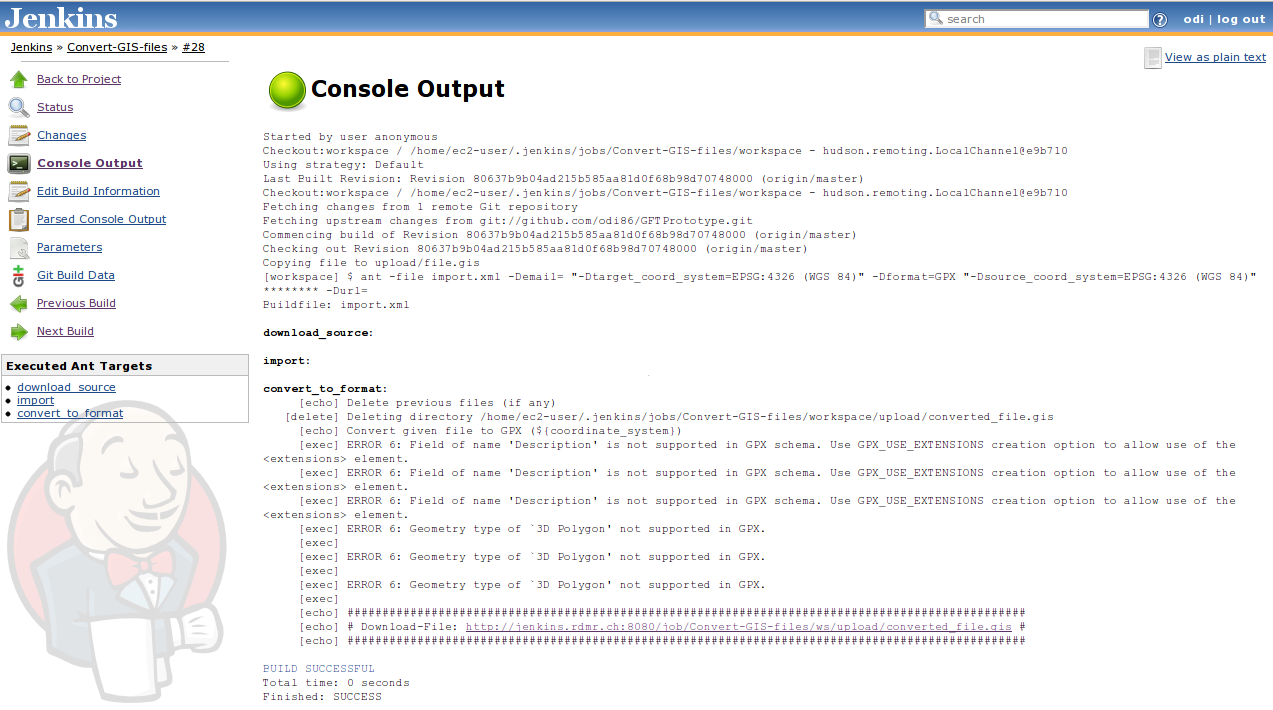
\includegraphics[width=\textwidth]{images/converter-build/converter-build-done}
	\caption{Konvertierung abgeschlossen}
	\label{converter-build-done}
\end{figure}

Als Quelldatei kann man wahlweise eine Datei hochladen oder eine URL auf eine Datei im Internet angeben. Weiter lässt sich das gewünschte Dateiformat und eine allfällige Koordinatenkonvertierung einstellen. Falls als Ausgabeformat \emph{GFT} gewählt wurde, muss man noch seine Angaben zu seinem Google-Konto angeben.

\begin{figure}[!ht]
	\centering
	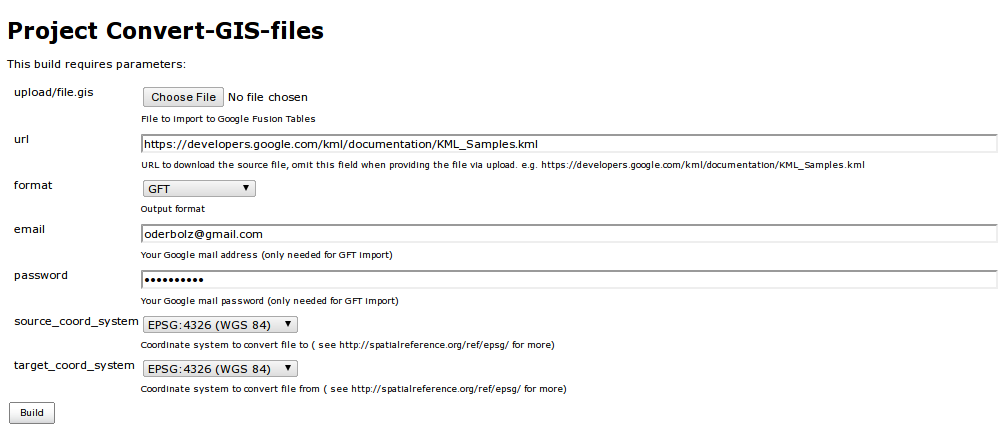
\includegraphics[width=\textwidth]{images/converter-build/converter-build-import}
	\caption{Optionen für den Converter-Build}
	\label{converter-build-import}
\end{figure}

\section{Installation}
Die Voraussetzungen für den Converter-Build sind zunächst eine Jenkins-Instanz, auf welcher das Plugin \emph{Parametetrized Build}\footnote{\url{https://wiki.jenkins-ci.org/display/JENKINS/Parameterized+Build}} installiert ist. Damit lassen sich an den Build via Web GUI Parameter übergeben. Grundsätzlich können damit generische Build-Jobs erstellt werden. 

Das Herzstück des Builds ist die GDAL/OGR Bibliothek welche sich aus dem Quellcode kompilieren lässt. Wichtig ist dabei, dass die Option \inlinecode{-{}-with-curl} angegeben wird, da ansonsten der GFT-Import nicht funktioniert.

\lstset{language=bash}
\begin{lstlisting}[caption=Kompilierung der GDAL/OGR Bibliothek mit cURL, label=converter-build-example]
$ ./configure --with-curl
$ make
# make install
\end{lstlisting}

Für die Koordinaten-Konvertierung muss zusätzlich noch die Bibliothek Proj.4\footnote{\url{http://trac.osgeo.org/proj/}} installiert werden.


% Neue Seite beginnen
\cleardoublepage

% Projektmanagement
% Titel auch in Kopfzeile anzeigen
\markboth{Teil IV. Projektmanagement und -monitoring}{Teil VI. Projektmanagement und -monitoring}
\part{Projektmanagement und -monitoring}
% Projektmanagement
\chapter{Projektmanagement}

\section{Allgemeines}

\section{Projektmanagement}

\section{Projektmonitoring}


% Projektmonitoring
\chapter{Projektmonitoring}
\label{projektmonitoring}

\section{Projektverlauf}
In Abbildung \ref{overall_stories_gantt_chart} sind alle erledigten Stories mit Start- und Endpunkt auf der Zeitachse abgebildet. Leider werden die Sprints etwas verfälscht dargestellt, da wir einzelne bereits begonnene Stories aus Zeitgründen von einem Sprint in den nächsten verschoben haben (Stories \#25, \#113 und \#186). Diese werden von Redmine dann über mehrere Sprints hinweg dargestellt, was natürlich auch den Sprint künstlich "`verlängert"'.

\begin{figure}[H]
	\centering
	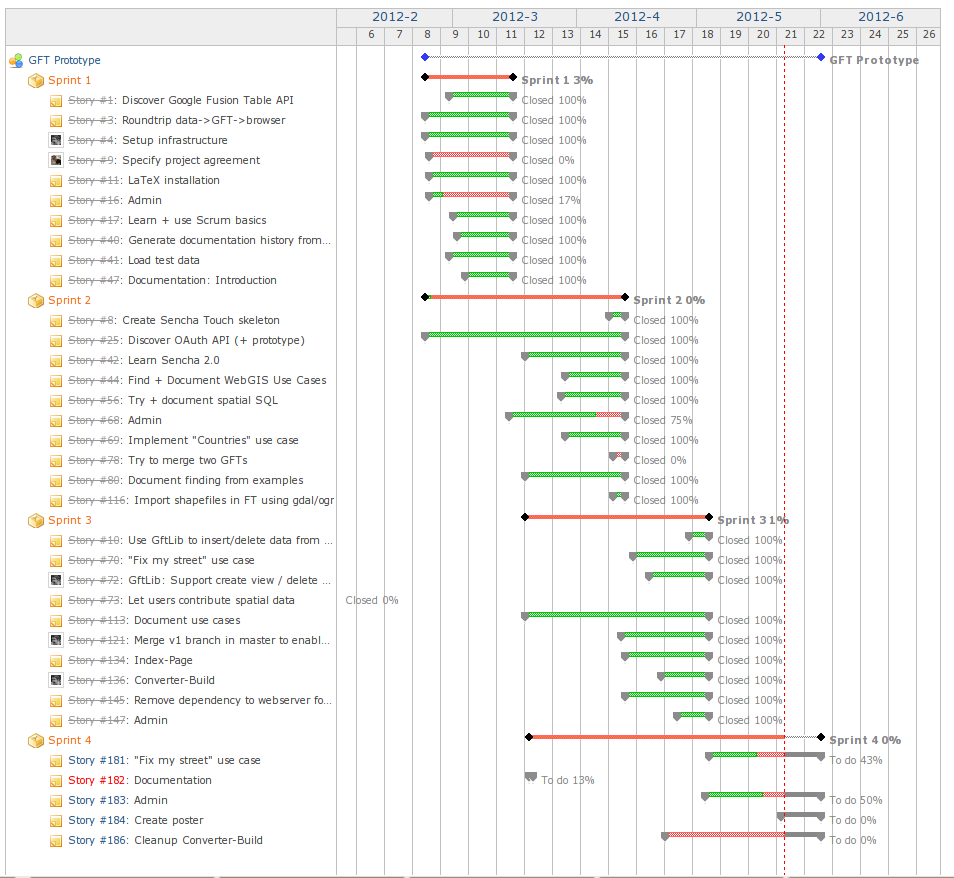
\includegraphics[width=\textwidth]{images/projektmanagement/overall_stories_gantt_chart}
	\caption{Gantt-Diagramm des Projektverlaufs}
	\label{overall_stories_gantt_chart}
\end{figure}

\section{Arbeitsaufwand}
Wie schon im Kapitel \ref{projektmanagement} beschrieben, war der vom Modul vorgegebene Aufwand pro Person auf \emph{240 Stunden} festgelegt. Wie in der Tabelle \ref{projektmanagement-arbeitsaufwand} ersichtlich haben wir diese Vorgabe beide leicht überschritten.

\begin{longtable}{|l|l|}
\hline 
\textbf{Person} & \textbf{Aufwand} \\ 
\hline 
Stefan Oderbolz & 255h \\ 
\hline 
Jürg Hunziker & 264h \\ 
\hline 
\caption{Arbeitsaufwand pro Person}
\label{projektmanagement-arbeitsaufwand}
\end{longtable} 

\section{Fazit}
Wir haben bezüglich Projektmanagement in diesem Projekt gute Erfahrungen mit Scrum sammeln können. Zuvor kannten wir diese Methodik lediglich aus der Theorie. Jetzt konnten wir die Stärken und Schwächen selbst kennenlernen.

Es ist klar, dass wir Scrum für unsere Bedürfnisse etwas anpassen mussten, gerade weil wir nur zwei Personen im Projektteam waren. Es hat sich bewährt jeweils Stories für neue Features im Backlog zu erfassen, wenn diese gerade aufgetaucht sind. Bei der Planung eines neuen Sprints konnten wir so die bestehenden Stories mit Schätzungen versehen und diese dann auf den Sprint planen.

Dank unserem Tooling mit Redmine hatten wir stets den Überblick über unser Projekt und die noch offenen Stories bzw. deren Tasks. Darin konnten wir auch gleich unsere Zeiterfassung unterbringen, indem wir unsere Aufwände auf die Tasks buchten. Das Projekt war hingegen fast zu kurz, um von den Stories Points zu profitieren. Wir haben über alle 4 Sprints hinweg mit durchschnittlich 12 Points pro Sprint gerechnet.


% -----------------------------------------
% FOOT
% -----------------------------------------
% Neue Seite beginnen
\cleardoublepage

% Anhänge
% Titel auch in Kopfzeile anzeigen
\markboth{Teil V. Anhänge}{Teil V. Anhänge}
\part{Anhänge}

% Inhalt der CD
\chapter*{Inhalt der CD}
% Titel auch in Kopfzeile anzeigen
\markboth{Inhalt der CD}{Inhalt der CD}
% Kapitel in Inhaltsverzeichnis einfügen
\addcontentsline{toc}{chapter}{Inhalt der CD}

\begin{longtable}{|p{0.35\twocelltabwidth}|p{0.65\twocelltabwidth}|}
\hline 
\textbf{Verzeichnis} & \textbf{Beschreibung} \\ 
\hline 
\inlinecode{SenchaDesignerProject/} & Beispielapplikation welche mit dem Sencha Designer erstellt wurde \\ 
\hline 
\inlinecode{\_DESIGN/} & Grafik-Rohdaten \\ 
\hline 
\inlinecode{\_DOCUMENTATION/} & Dokumentation der Arbeit \\ 
\hline 
\inlinecode{classes/} & PHP Serverklassen \\ 
\hline 
\inlinecode{examples/} & Beispielapplikationen \\ 
\hline 
\inlinecode{lib/} & Verwendete Library-Pakete \\ 
\hline 
\inlinecode{resources/} & Ressourcen, welche für die Indexseite verwendet wurden (CSS, Bilder) \\ 
\hline 
\inlinecode{services/} & PHP Webservices \\ 
\hline 
\inlinecode{test/} & Tests der Use Cases und Libraries \\ 
\hline 
\inlinecode{usecases/} & Use Cases welche implementiert wurden (WorldData, FixMyStreet) \\ 
\hline 
\end{longtable} 

% Glossar
\printglossary[style=altlist,title=Glossar,toctitle=Glossar]

% Literaturverzeichnis
\bibliographystyle{plainurl}
\bibliography{foot/literatur}

% Abbildungsverzeichnis
\listoffigures

% Tabellenverzeichnis
\listoftables

\end{document}